\documentclass[10pt]{beamer}

\usetheme{metropolis}
\usepackage{appendixnumberbeamer}

\usepackage{booktabs}
\usepackage[scale=2]{ccicons}
\usepackage{amsmath}
\usepackage{xspace}
\usepackage{graphicx}
\usepackage{subfigure}
\graphicspath{{Graphics/}}


\newcommand{\themename}{\textbf{\textsc{metropolis}}\xspace}

\title{High Order Positivity Preserving Finite Difference Scheme for Compressible Two Fluid/Phase Flow Model}
% \subtitle{Thesis Research - Overview}

%\subtitle{Validation}
\date{\today}
\author{Daniel Boe, Khosro Shahbazi}
\institute{South Dakota School of Mines and Technology}

\begin{document}

\maketitle

\begin{frame}{Overview}
  \begin{itemize}
  \item Introduction - Applications, Challenges, and Objectives
  \item Overview of model
  \item Methodology
  \item Numerical Examples
  \item Conclusion
  \end{itemize}
  \end{frame}

  \begin{frame}{Applications}
    \textbf{Two phase/fluid dynamics occur in numerous fields}
    \begin{itemize}
      \item Sustainable Energy / cooling systems
      \item Defense
      \item Healthcare
      \begin{itemize}
        \item[o] Treatment Modeling
        \begin{itemize}
          \item Laser-activated Perflourocarbon nanodroplets (PFCnD)
        \end{itemize} 
        \item[o] Cold Chain equipment
        \begin{itemize}
          \item Portable vapor-compression systems
          \item Mobile absorption based systems (Einstein refrigerator, ``Icyball'')
          \item Switchable adsorption/zeolite refrigeration systems
        \end{itemize} 
      \end{itemize}
      \item Volcanology
        \begin{itemize}
          \item[o] Vulcanian eruptions
        \end{itemize}
    \end{itemize}
  \end{frame}

  \begin{frame}{Challanges}
\textbf{Two phase/fluid problems are characterized by physical phenomena that pose significant challenges to numerical algorithms.}
  \begin{itemize}
    \item Highly nonlinear (shock waves, and high-intensity ultrasound waves)
    \item Complex wave propagation and high-frequency features
        \begin{itemize}
          \item[o] \textit{Demands high fidelity numerical algorithm to accurately capture}
        \end{itemize}
    \item Large, discontinuous jumps across shocks and even larger jumps across material interfaces
        \begin{itemize}
          \item[o] \textit{Requires non-oscillatory, positivity preserving scheme to ensure physical integrity}
        \end{itemize}
  \end{itemize}
  \textbf{Failure to maintain positivity of density and the square of sound speed leads to the simulation crashing}  
  \end{frame}

  \begin{frame}{Objectives}
    \textbf{The objectives are to design, analyze and implement numerical schemes applicable to general compressible multiphase dynamics satisfying}
    \begin{enumerate}
      \item Hyperbolicity (real Eigenvalues/characteristic speeds)
      \item High order
      \item Non-oscillatory
      \item Positivity-preserving
      \item High efficiency, simplicity and scalability on parallel
      computers
    \end{enumerate}
  \end{frame}

\begin{frame}{Conservation Law}
  \begin{itemize}
    \item  In a closed system, the overall quantity of some property can only change by adding or removing this property. 
    \item Enforces fundamental principle that forms the basis for modeling numerous physical processes. 
  \end{itemize} 

  \begin{equation}
    \frac{\partial u(x,t)}{\partial t} + \frac{\partial}{\partial x}[f(u(x,t))]=0\label{eq:Conservation Law}
  \end{equation}
  
  where 
  \begin{itemize}
    \item $u(x,t)$ is a function describing the distribution of some physical quantity 
    \item $f$ is a function giving the flux of the conserved quantity.
  \end{itemize}

\end{frame}

\begin{frame}{Euler Equations}
  \begin{align}
    \frac{\partial \rho}{\partial t}+\frac{\partial}{\partial x}[\rho v] &=0\label{eq:MassBalance}\\
    \frac{\partial}{\partial t}[\rho v]+\frac{\partial}{\partial x}[\rho v^2+p]&=0\label{eq:MomentaBalance}\\
    \frac{\partial}{\partial t}[\rho(e+\tfrac{v^2}{2})]+\frac{\partial}{\partial x}[(\rho e+\tfrac{\rho v^2}{2} +p)v]&=0\label{eq:EnergyBalance}
    \end{align} 
  \begin{itemize}
    \item Ideal Gas Law gives $e\rho(\gamma -1)=p$
    \begin{itemize}
      \item[o] $e$ is specific internal energy.  
      \item[o] $\gamma$ specific heat ratio $\frac{c_p}{c_v}$
    \end{itemize}
    \item $\textbf{u}=[\rho,\rho v,\rho(e+\tfrac{v^2}{2})]^T$
    \begin{itemize}
      \item[o] vector of \textit{conserved} variables - specific density, specific momentum, and specific total energy. 
    \end{itemize}
    \item $\textbf{u}_p=[\rho,v, p]^T$
    \begin{itemize}
      \item[o] vector of \textit{primitive} variables - density, velocity, and pressure
    \end{itemize}
    \item $\textbf{f} = [\rho v, \rho v^2 + p, (\rho(e+\tfrac{\rho v^2}{2})+p)v]^T$
    \begin{itemize}
      \item[o] vector of fluxes
    \end{itemize}
  \end{itemize}
\end{frame}


\begin{frame}{Two Fluid System}
  The Euler equations can be extended to a two-fluid system by adding two additional equations.
  \begin{align}
    \frac{\partial \Gamma_1 }{\partial t} + \frac{\partial}{\partial x}[v\Gamma_1] - \Gamma_1 \frac{\partial v}{\partial x}&=0\label{eq: Order Parameter One}\\
    \frac{\partial \Gamma_2 }{\partial t} + \frac{\partial}{\partial x}[v\Gamma_2] - \Gamma_1 \frac{\partial v}{\partial x}&=0\label{eq: Order Parameter Two}
  \end{align}

  \begin{itemize}
    \item $\Gamma_1 = \frac{1}{\gamma -1}$ and $\Gamma_2 = \frac{\gamma \Pi}{\gamma -1}$ are interface capturing functions
    \item Stiffened Gas Equation of State: $p = e\rho(\gamma - 1) -\gamma \Pi$
    \begin{itemize}
      \item[o] Provides a means of modeling state for both liquid and gas 
      \item[o] $\Pi$ is empirical parameter
      \begin{itemize}
        \item [-] $\Pi = 0$ for ideal gas
        \item [-] $\Pi \approx 4(10^8)$ for liquid water
      \end{itemize}    
    \end{itemize}
  \end{itemize}

\end{frame}

% \begin{frame}{Model Summary}
%   \begin{align}
%     \frac{\partial \rho}{\partial t}+\frac{\partial}{\partial x}[\rho v] &=0\label{eq:MassBalance}\\
%     \frac{\partial}{\partial t}[\rho v]+\frac{\partial}{\partial x}[\rho v^2+p]&=0\label{eq:MomentaBalance}\\
%     \frac{\partial}{\partial t}[\rho(e+\tfrac{v^2}{2})]+\frac{\partial}{\partial x}[(\rho e+\tfrac{\rho v^2}{2} +p)v]&=0\label{eq:EnergyBalance}\\
%     \frac{\partial \Gamma_1 }{\partial t} + \frac{\partial}{\partial x}[v\Gamma_1] - \Gamma_1 \frac{\partial v}{\partial x}&=0\label{eq: Order Parameter One}\\
%     \frac{\partial \Gamma_2 }{\partial t} + \frac{\partial}{\partial x}[v\Gamma_2] - \Gamma_1 \frac{\partial v}{\partial x}&=0\label{eq: Order Parameter Two}\\
%     e\rho(\gamma - 1) -\gamma \Pi &=p\\
%     \Gamma_1 &= \frac{1}{\gamma -1}\\
%     \Gamma_2 &= \frac{\gamma \Pi}{\gamma -1}
%     \end{align} 
% \end{frame}

\begin{frame}{Model Summary}
  \centering
\textbf{We need to solve the following model subject to shocks, oscillations, and discontinuities:}
\centering
  \begin{align}
    \frac{\partial \rho}{\partial t}+\frac{\partial}{\partial x}[\rho v] &=0 \nonumber\\
    \frac{\partial}{\partial t}[\rho v]+\frac{\partial}{\partial x}[\rho v^2+p]&=0 \nonumber \\
    \frac{\partial}{\partial t}[\rho(e+\tfrac{v^2}{2})]+\frac{\partial}{\partial x}[(\rho e+\tfrac{\rho v^2}{2} +p)v]&=0 \nonumber\\
    \frac{\partial \Gamma_1 }{\partial t} + \frac{\partial}{\partial x}[v\Gamma_1] - \Gamma_1 \frac{\partial v}{\partial x}&=0 \nonumber\\
    \frac{\partial \Gamma_2 }{\partial t} + \frac{\partial}{\partial x}[v\Gamma_2] - \Gamma_1 \frac{\partial v}{\partial x}&=0 \nonumber \\
    e\rho(\gamma - 1) -\gamma \Pi &=p \nonumber
    \end{align} 
\end{frame}







\begin{frame}{Finite Difference Schemes}
\textbf{Why Finite Difference Schemes?}
\begin{itemize}
\item Able to capture shock discontinuities prevalent in CFD
\item Well suited for multi-scale phenomena associated with multi-phase/multi-fluid dynamics.
\item Unmatched simplicity and efficiency
\end{itemize}
\textbf{Why High Order Schemes?}
\begin{itemize}
\item High order schemes allow for greater accuracy per CPU cost (KS, JCP, 2017) \cite{Shahbazi2017,Shahbazi}
\begin{itemize}
\item[--] Enhances ability to solve multi-dimensional problems
\end{itemize}
\end{itemize}
\end{frame}

% GOOD Reference, but likely not within time constraints for this presentation

% \begin{frame}{Finite Difference Schemes}
%   The Taylor Series expansion $u(x)$ centered about $x_i$ evaluated at $x=x_i + jh$ is:
%   \begin{equation}
%     u(x_i+jh)=u(x_i)+(jh)\frac{d u}{dx}\bigg|_{x_i}+\frac{(jh)^2}{2!}\frac{d^2u}{dx^2}\bigg|_{x_i} + \frac{(jh)^3}{3!}\frac{d^3u}{dx^3}\bigg|_{x_i} + \mathcal{O}(h^4)
%   \end{equation}
%   taking $j=1$, we have 
%   \begin{equation}
%     u(x_i+h)=u(x_i)+(h)\frac{d u}{dx}\bigg|_{x_i}+ \frac{1}{2!}\frac{d^2u}{dx^2}\bigg|_{x_i}+ \mathcal{O}(h^3)
%   \end{equation}
%   Truncating the higher order terms and solving for the derivative gives:
%   \begin{equation}
%     \frac{d u}{dx}\bigg|_{x_i} \approx \frac{u(x_i+h) - u(x_i)}{h} = \frac{u_{i+1} - u_i}{h}
%   \end{equation}
%   which is a first order, \textit{forward} finite difference approximation.
%   \begin{itemize}
%     \item It is a forward-biased approximation because we utilize a point ($x_{i+1}$) that falls after or downwind of $x_i$ on the grid.
%     \item Taking $j=-1$ would give a backwards finite difference formula.
%     \item Subtracting the backwards scheme from the forward scheme would cancel the second derivative term to give a second order approximation.
%   \end{itemize}
% \end{frame}


\begin{frame}{Higher Order Schemes}
  %% This paragraph is coupled with the previous slide (which I am probably throwing out)
  % High order finite difference approximations can be obtained by evaluating the Taylor expansion at multiple points surrounding $x_i$ and combining each approximation such that the $2^{nd}, 3^{rd}, 4^{th} \dots $ order terms cancel. 
  \centering 
  \textbf{High order schemes offer superior accuracy per CPU cost}
  
  \begin{table}[H]
    \centering
      \tabcolsep=0.3cm
      \scalebox{0.55}{
  \begin{tabular}{lll}
    \toprule
     &         First Order        &          Fifth Order   \\
     & N=1600 Grid Points         &          N=50 Grid Points \\
    \midrule
    $L_{\infty}$ Error \% &      4.86\% &     0.13\%             \\
    CPU Time [sec] &      	0.32 &        	0.20        \\
    \bottomrule
    \end{tabular}}
  \end{table}
  \begin{figure}[H]
      \centering
      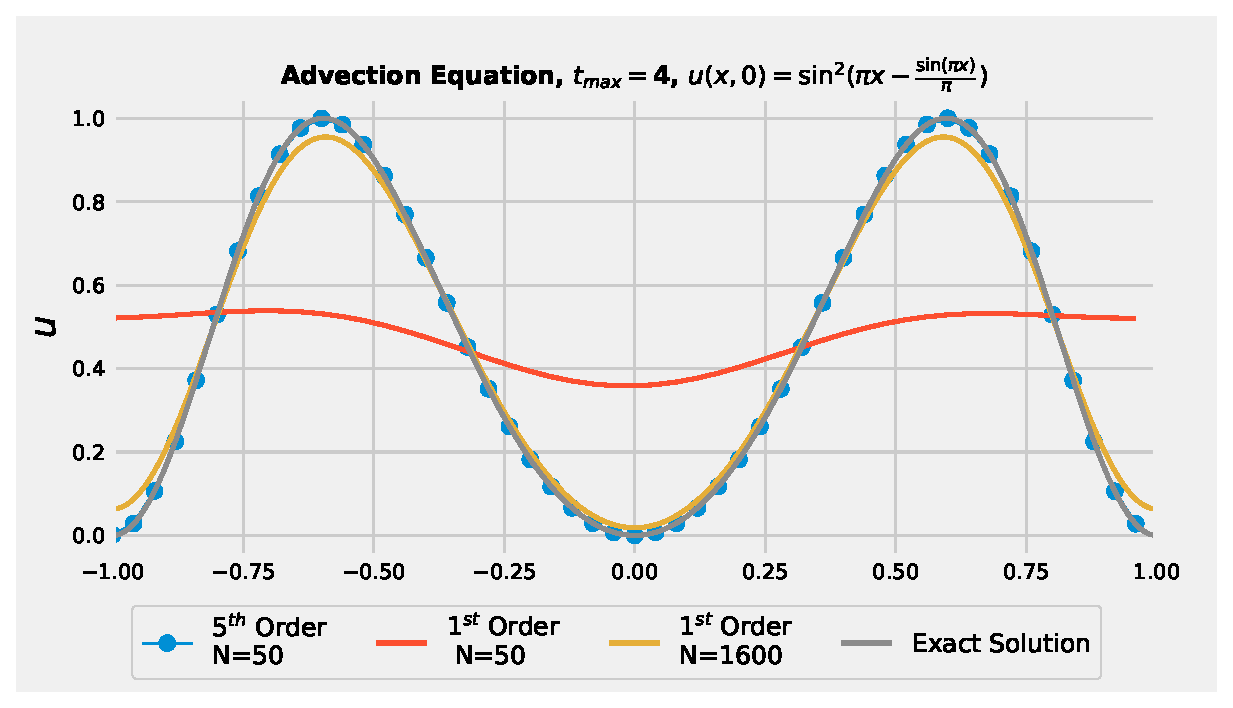
\includegraphics[scale=0.45]{AdvectionHighOrderComparison2.eps}
    \end{figure}
\end{frame}


\begin{frame}{Discontinuous Solutions}
  \centering
  \textbf{For discontinuous solutions, high order methods suffer from spurious oscillations that do not diminish with grid refinement.}
  
  \begin{figure}[H]
    \centering
    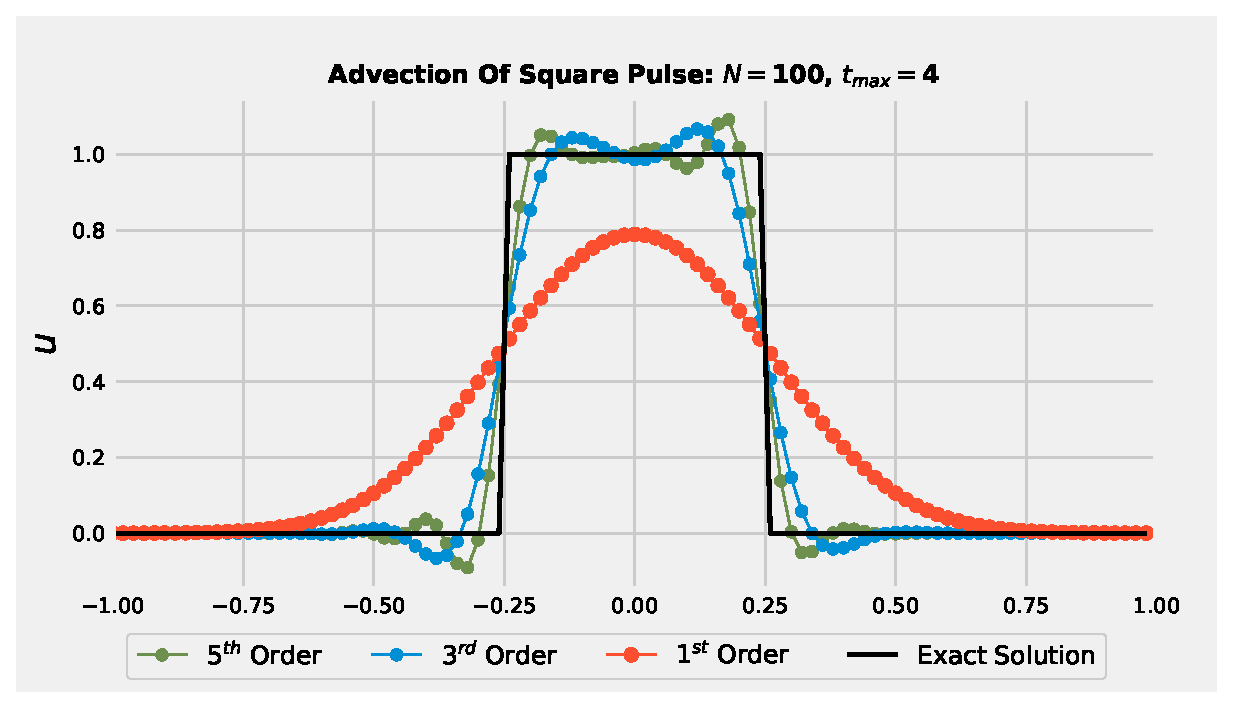
\includegraphics[scale=0.45]{AdvectionHighOrderComparison_pulse.eps}
    \end{figure}
\end{frame}

\begin{frame}{Non Linear Scheme}
  \textbf{To obtain a robust algorithm, we need a globally high order, non-linear scheme that can locally adapt to discontinuous solutions}
\end{frame}


\begin{frame}{Discretization}
  We seek a non-linear scheme for the discrete conservation law
  \begin{equation}
    \frac{\partial}{\partial t}[u_i^n] + \frac{\partial}{\partial x}[f(u_i^n)] = 0
  \end{equation}
  where 
  \begin{itemize}
    \item Domain is $[x_{min},x_{max}] \times [0,t_{max}]$
    \begin{figure}[H]
      \centering
      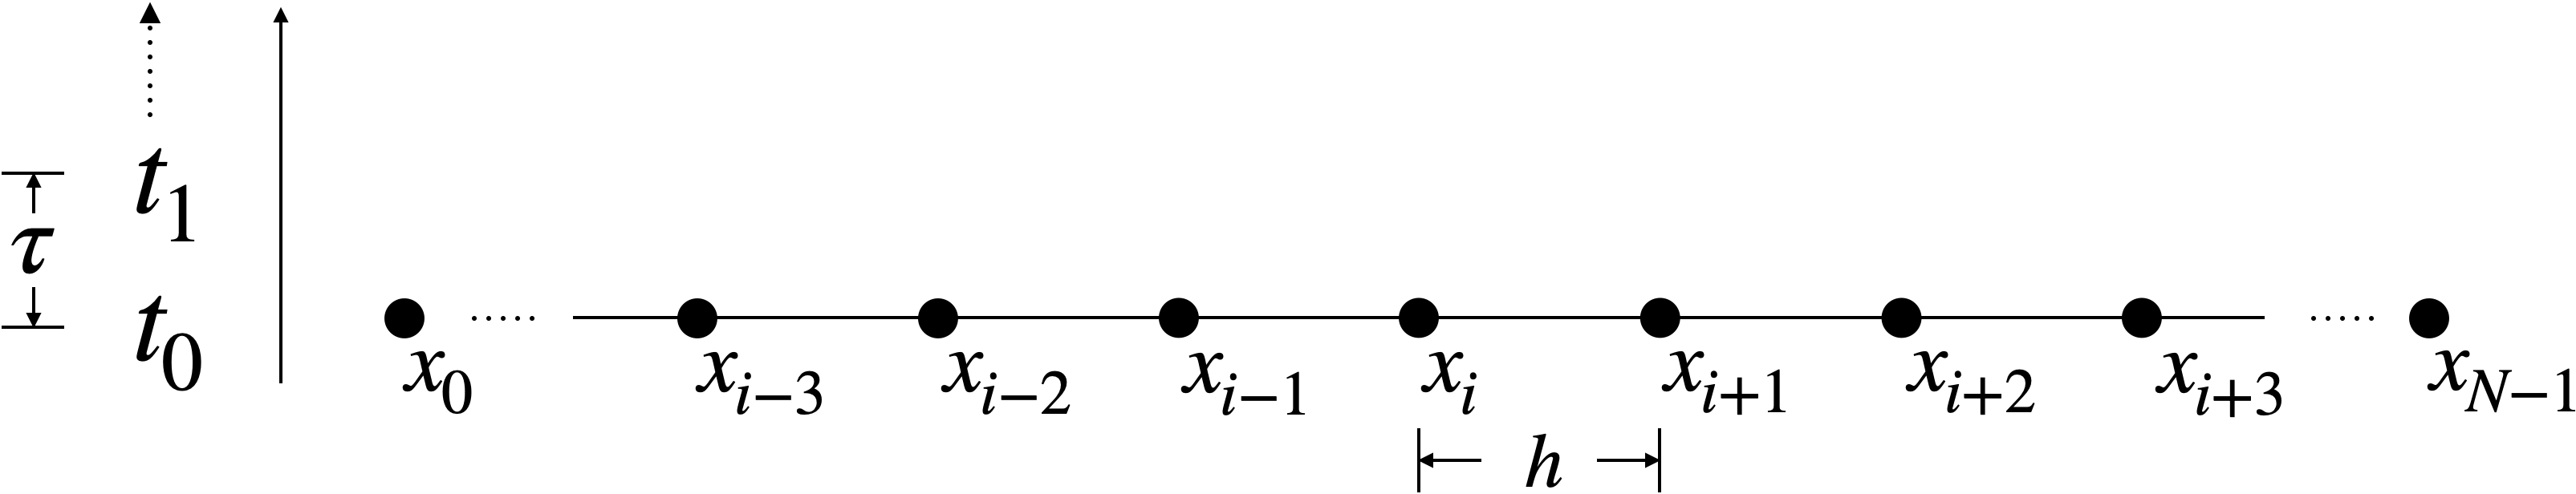
\includegraphics[scale=0.175]{GridGraphic_time.png}
    \end{figure}
    \item $u_i = u(x_i)$ is the conserved variable evaluated at the gridpoint $x_i$ at time step $n$
    \begin{itemize}
      \item[o]  $i \in \{0,1,2 \dots N-1\}$ with $N$ being the total number of cells
      \item[o] $h = \frac{x_{max} - x_{min}}{N}$ is the step size in-between adjacent cells
    \end{itemize}
  \end{itemize}
\end{frame}

% \begin{frame}{Conservation Laws with Discontinuous Data}
%   \textbf{Why Non-Linear Schemes?}
%   \begin{itemize}
%   \item High order Finite Difference schemes suffer from spurious oscillations near discontinuities
%   \item Non-linear methods attenuate oscillations by utilizing a feedback loop to adjust the solution scheme near discontinuities
%   \begin{itemize}
%   \item[--] High order solution is retained in smooth regions 
%   \item[--] First order, non-oscillatory solution is obtained in discontinuous regions
%   \end{itemize}
%   \end{itemize}
% \end{frame}

% \begin{frame}{WENO scheme}
%   \textbf{WENO Method}  
%   \newline Assume the spatial derivative term can be written exactly as the difference of some ``numerical flux function" evaluated at the cell boundaries.
%   \begin{equation}
%     \frac{\partial}{\partial x}[f(u_i)] = \frac{\bar{f}_{i+1 /2} - \bar{f}_{i-1/2}}{h}
%   \end{equation}
%   where
%   \begin{equation}
%     f(u_i)=\frac{1}{h}\int_{x-h/2}^{x+h/2} \bar{f}(\xi)d\xi
%   \end{equation}
%   \begin{itemize}
%   \item Thus, the goal of the WENO scheme is to develop high order, non-oscillatory approximations for the numerical flux function $\bar{f}_{i\pm1/2}$
%   \item The numerical flux function can be computed from the known flux $f(u_i)$
%   % \item Technically, WENO is not, in itself, a finite difference scheme; rather it is a method of flux reconstruction. \cite{Jiang96,Henrick05}
%   \end{itemize}
%   \end{frame}





\begin{frame}{Approach}
\begin{columns}
  \begin{column}{0.65\textwidth}
    From divergence theorem, we can relate the derivative term at $x_i$ to the fluxes into and out of the cell $I_i$.
    $$
      \frac{\partial}{\partial x}[f(u_i)] \approx \frac{\hat{f}_{i+1 /2} - \hat{f}_{i-1/2}}{h}
    $$
    \textbf{Our goal}:

  High order, non-oscillatory approximations to the cell boundary fluxes, $f(u(x_{i\pm1/2}))$  
  \end{column}

  \begin{column}{0.3\textwidth}
  \vspace{\topsep}
  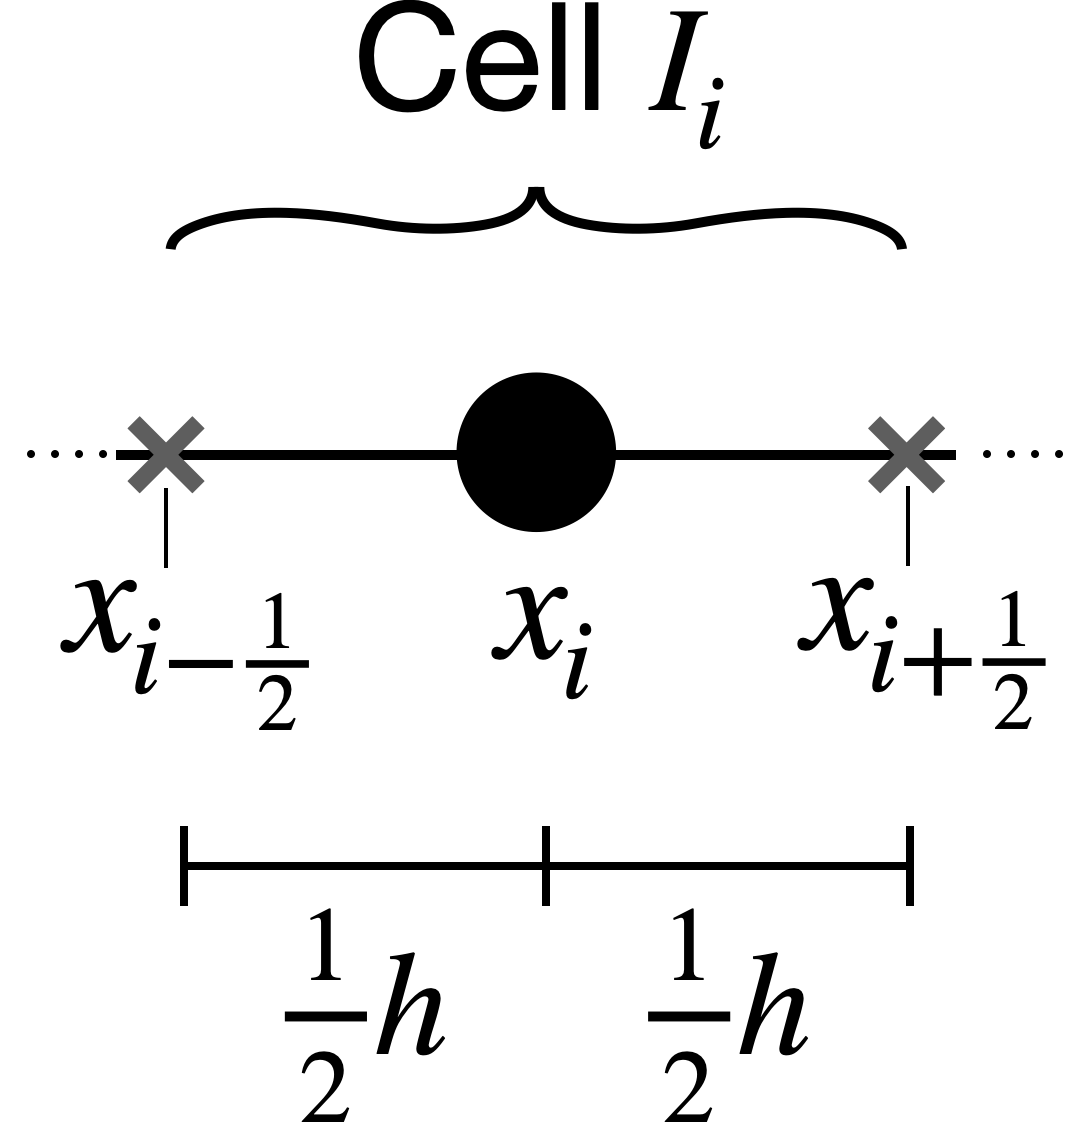
\includegraphics[scale=0.175]{CellGraphic.png}%
  \end{column}
    
  \end{columns}
\end{frame}



  \begin{frame}{The Plan}
    \textbf{Weighted Essentially Non Oscillatory (WENO) Method}
    \begin{enumerate}
      \item Calculate local polynomial approximation at each stencil
      \item Measure the smoothness of each polynomial approximation
      \item Form a weighted sum of all the approximations
          \begin{itemize}
            \item[o] Stencil weight is proportional to smoothness
            \item[o] Discontinuous stencils assigned weight $\rightarrow$ 0
            \item[o] Smooth stencils assigned an optimal weight 
            \item[o] If all stencils are smooth, overall approximation is of optimal order. 
          \end{itemize}
    \end{enumerate}


    \begin{figure}[H]
      \centering
      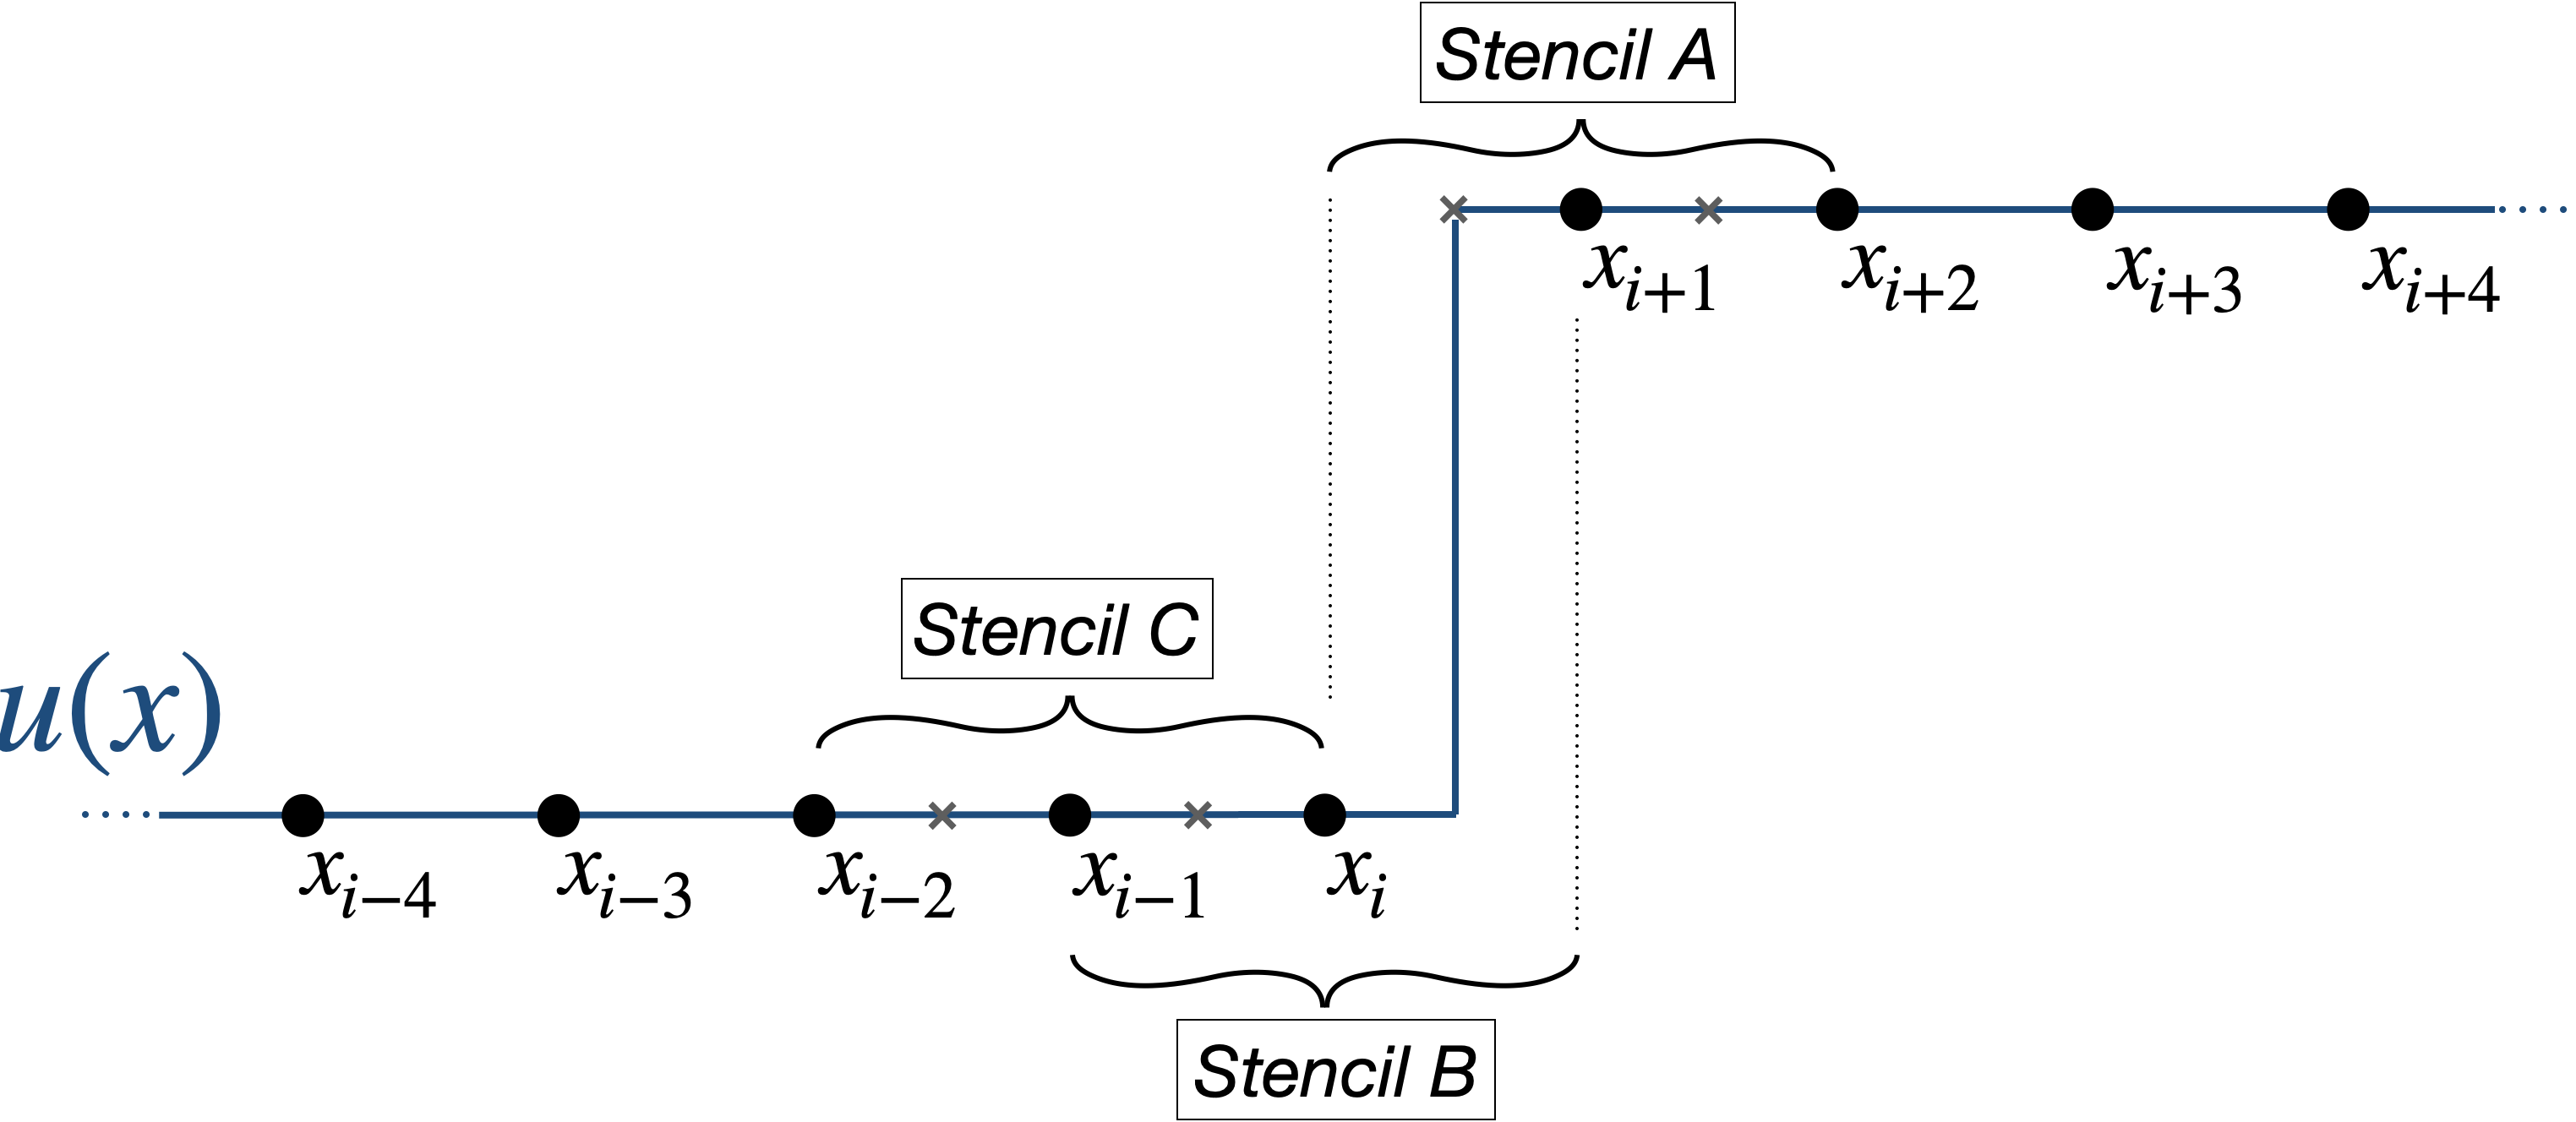
\includegraphics[scale=0.175]{DiscontinuousStencil.png}
      \end{figure}
  \end{frame}


\begin{frame}{WENO Implementation}
  The WENO reconstruction of $u(x_{i+1/2})$ takes the form:
  \begin{equation}
    u(x_{i+1/2})\approx P^{WENO}_{i+\frac{1}{2}}=\sum_{k=0}^{r-1}\omega_{k,i+\frac{1}{2}}P_{k,i+\frac{1}{2}}\label{eq:WenoEquation}
  \end{equation}
  where $\omega_{k,i+\frac{1}{2}}$ is the normalization of the non-linear weights:
  \begin{align}
    \alpha_{k,i+\frac{1}{2}}&=\frac{b_{r,k}}{(\beta_{k,i+\frac{1}{2}} +10^{-40})^r}
  \end{align}
  $b_{r,k}$ are the optimal linear weights and 
  $\beta_{r,k_s,i}$ are the smoothness indicators
  \begin{equation}
    \beta_{k,i} = \sum_{l=0}^{r-1}h^{2m-1}\int_{-\frac{1}{2}h}^{\frac{1}{2}h}\bigg[\frac{d^m}{d\xi}P_{k,i+1/2}(\xi)\bigg]^2d(\xi-x_i)\label{eq:OptimalCoefficients}
  \end{equation}
\end{frame}

% \begin{frame}{WENO Framework}
%   For an arbitrary function $u(x_i)$, we can form an $r^{th}$ order, polynomial representation of $u(x_{i+1/2})$ as:
%   \begin{equation}
%     u(x_i+\tfrac{1}{2}h) \approx P_{r,k_s,i+\frac{1}{2}}= \sum_{q=0}^{q=r-1}a_{r,k_s,q}u_{i-k_s+q}\label{eq:PolynomialReconstruction}
%   \end{equation}
%   where $a_{r,k_s,q}$ are tabulated constants for a given order ($r$), stencil ($k_s$), and stencil cell ($q$).
%   \begin{figure}[H]
%     \centering
%     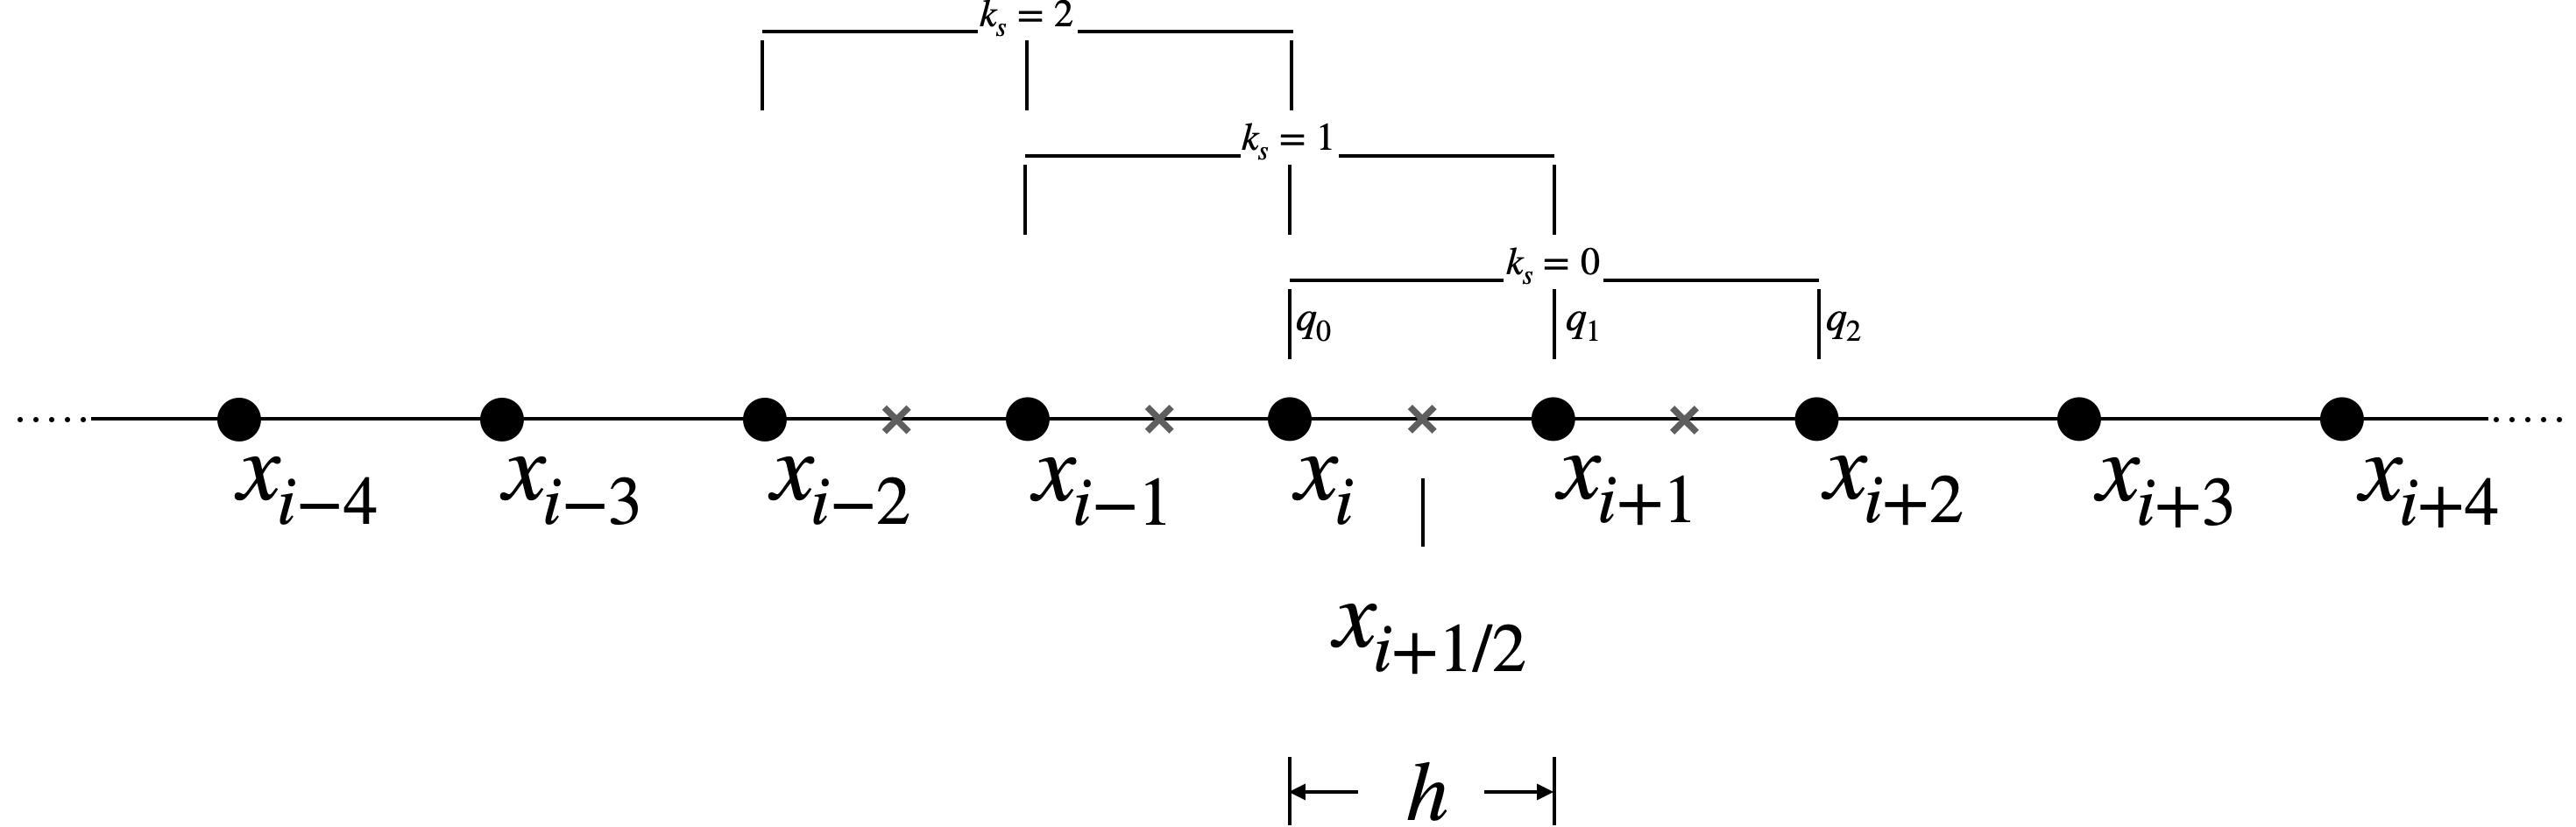
\includegraphics[scale=0.165]{StencilReconstruct.png}\caption{Illustration of candidate stencils for forming $P_{r,k_s,i+1/2}$}
%       \label{fig: Stencil Graphic}
%   \end{figure}
% \end{frame}

% \begin{frame}{WENO Framework}
%   By properly combining the polynomials associated with each candidate stencil, we can construct a $2r-1$ order approximation for $u(x_{i+1/2})$
%   \begin{equation}
%     P^{*}_{r,i+\frac{1}{2}} = \sum_{k_s=0}^{k_s=r-1}b_{r,k_s}P_{r,k_s,i+\frac{1}{2}}\label{eq: Optimal Reconstruction Definition}
%   \end{equation}
%   Here, $b_{r,k_s}$ are tabulated weights assigned to the local, $r^{th}$ order polynomial associated with sub-stencil $k_s$.
  
%   \begin{itemize}
%     \item The heart of WENO involves modifying the above approximation such that:
%     \begin{enumerate}
%       \item If sub-stencil $k_s$ contains a discontinuity, the weight $b_{r,k_s} \longrightarrow 0$ effectively negating the impacts of the discontinuity.
%       \item If no sub-stencils contain discontinuities, the above $2r-1$ order approximation is recovered.
%     \end{enumerate}
%   \end{itemize}
% \end{frame}

% \begin{frame}{WENO Framework}
%   The WENO reconstruction of $u(x_{i+1/2})$ takes the form:
%   \begin{equation}
%     P^{WENO}_{r,i+\frac{1}{2}}=\sum_{k_s=0}^{k_s=r-1}\omega_{r,k_s,i+\frac{1}{2}}P_{r,k_s,i+\frac{1}{2}}\label{eq:WenoEquation}
%   \end{equation}
%   where 
%   \begin{align}
%     \omega_{r,k_s}&=\frac{\alpha_{r,k_s}}{\sum_{j=0}^R\alpha_{r,j}}\\
%     \alpha_{r,k_s}&=\frac{b_{r,k_s}}{(\beta_{r,k_s,i} +10^{-40})^r}
%   \end{align}
%   define the WENO weights in terms of the linear, ``optimal weights'' ($b_{r,k_s}$) and a non-linear smoothness indicator $\beta_{r,k_s,i}$ which is defined as the sum of the $L^2$ norms of all derivatives of the original interpolating polynomial associated with the $k_s$ sub-stencil \cite{Jiang96}. 
%   \begin{equation}
%     \beta_{r,k_s,i} = \sum_{l=0}^{r-1}h^{2m-1}\int_{-\frac{1}{2}h}^{\frac{1}{2}h}\bigg[\frac{d^m}{d\xi}P_{r,k_s,i+1/2}(\xi)\bigg]^2d(\xi-x_i)\label{eq:OptimalCoefficients}
%   \end{equation}
% \end{frame}

% \begin{frame}{WENO Framework Summary}
%   The WENO process can be thought of as an operator, $L$, that takes a function $w(x_i)$ defined on a grid $x_i \in \{x_0, x_1 \dots x_{N-1}
%   \}$ and computes a $2r-1$ order polynomial approximation of $w$ at the intercell points $x_{i+1/2}$.
%   $$L(w_{i}) = \hat{w}_{{i+\frac{1}{2}}}\approx w_{{i+\frac{1}{2}}}$$
%   The basic steps for a $2r-1$ order approximation are:
%   \begin{enumerate}
%     \item Calculate the $r$ local polynomials: $P_{r,k_s,i+\frac{1}{2}}= \sum_{q=0}^{q=r-1}a_{r,k_s,q}w_{i-k_s+q}$
%     \item For each $P_{r,k_s,i+\frac{1}{2}}$, calculate the WENO smoothness indicators $\beta_{r,k_s,i}$.
%     \begin{itemize}
%       \item[o] These calculations are tabulated in the literature
%     \end{itemize}
%     \item Assemble the WENO weights, $\omega_{r,k_s}$, from the constant optimal weights $b_{r,k_s}$ and the non-linear weights $\beta_{r,k_s,i}$. 
%     \item Calculate the WENO polynomial: $\hat{w}_{i+1/2}=\sum_{k_s=0}^{k_s=r-1}\omega_{r,k_s,i+\frac{1}{2}}P_{r,k_s,i+\frac{1}{2}}$
%   \end{enumerate}
% \end{frame}

% \begin{frame}{WENO Implementation}
%   The WENO scheme provides a method for forming non-oscillatory approximations to the numerical flux function $\bar{f}_{i\pm 1/2}$. 
% \begin{itemize}
%   \item In general, the WENO reconstruction of the original flux $f$ gives this high order approximation.
%   $$\bar{f}_{i+1/2} \approx \hat{f}_{i+1/2} = L(f(u_i))$$
%   % \item  Performing the reconstruction on the known fluxes supplies the high order derivative approximation as:
%   % $$\frac{\partial}{\partial x}[f(u_i)] \approx \frac{\hat{f}_{i+1 /2} - \hat{f}_{i-1/2}}{h}$$
%   \item Alternately, the WENO reconstruction can be performed \textit{directly} upon the primitive variables (or conservative variable in the scalar case).
%   $$\bar{f}_{i+1/2} \approx f(\hat{u}_{i+1/2}) = f(L(u_i))$$
%   \begin{itemize}
%     \item[o] With this scheme, the spatial derivative is calculated with tabulated constants ($d_j$) as \cite{Shahbazi}:
%     $$	h\frac{\partial f}{\partial x}\bigg|_{x_i}\approx \sum_{j=1}^{j=\text{ceil}(\tfrac{r}{2})}d_j(f(\hat{u}_{i+j-1/2})-f(\hat{u}_{i-j-1/2}))$$
%   \end{itemize}
% \end{itemize}
% \end{frame}

\begin{frame}{WENO Summary}
  The WENO scheme provides a method for forming non-oscillatory approximations to primitive variables at cell boundaries.
  $$
  \hat{u}_{i+\frac{1}{2}} \approx u(x_{i}+\tfrac{1}{2}h)
  $$
  The derivative is then approximated to high order using constants $d_j$ introduced and tabulated to 9$^{th}$ order by Shahbazi (Computers and Fluids, 2019) and extended to 13$^{th}$ order (DB and KS, unpublished).
  $$	h\frac{\partial f}{\partial x}\bigg|_{x_i}\approx \sum_{j=1}^{j=\text{ceil}(\tfrac{r}{2})}d_j(f(\hat{u}_{i+j-1/2})-f(\hat{u}_{i-j-1/2}))$$
\end{frame}

\begin{frame}{Non-Linear Scheme for Advected Pulse}
  \centering
  \textbf{WENO scheme significantly reduces the spurious oscillations}
  \begin{figure}[H]
    \centering
    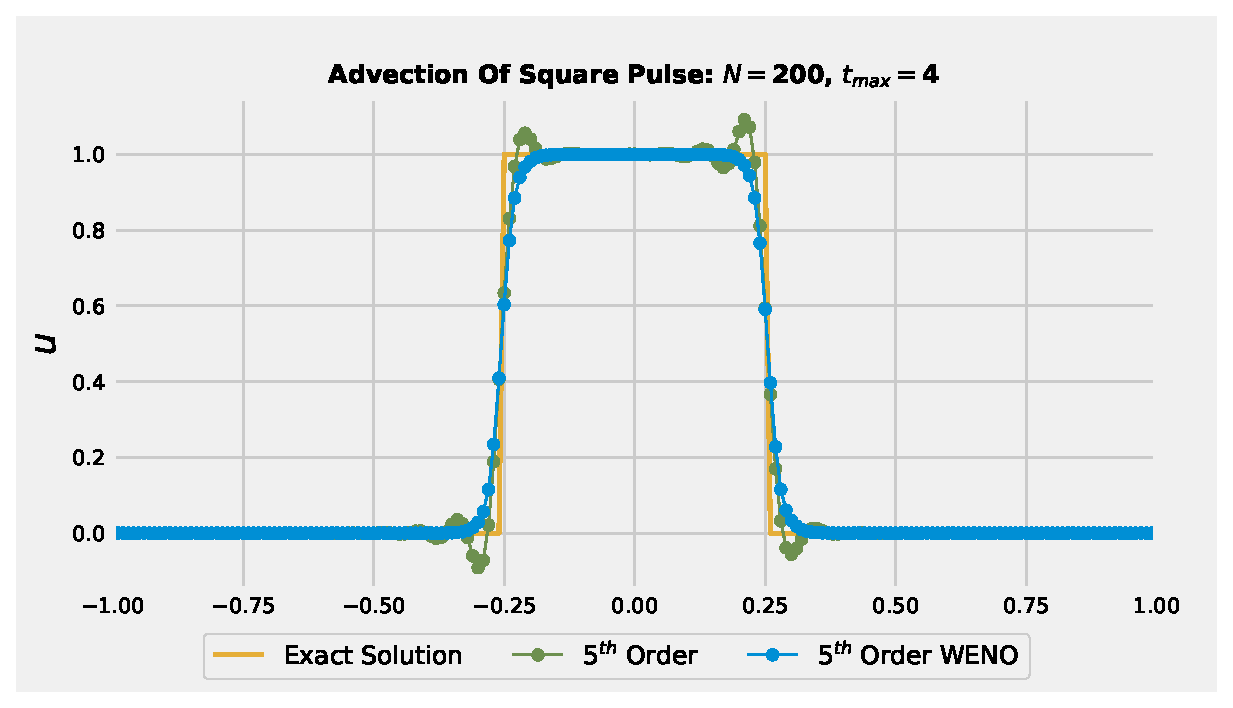
\includegraphics[scale=0.475]{AdvectionHighOrderComparison_pulseWENO.eps}
    \end{figure}
\end{frame}

\begin{frame}{Non-linear Scheme for Euler System}
  % \begin{figure}[H]
  %   \centering
  %   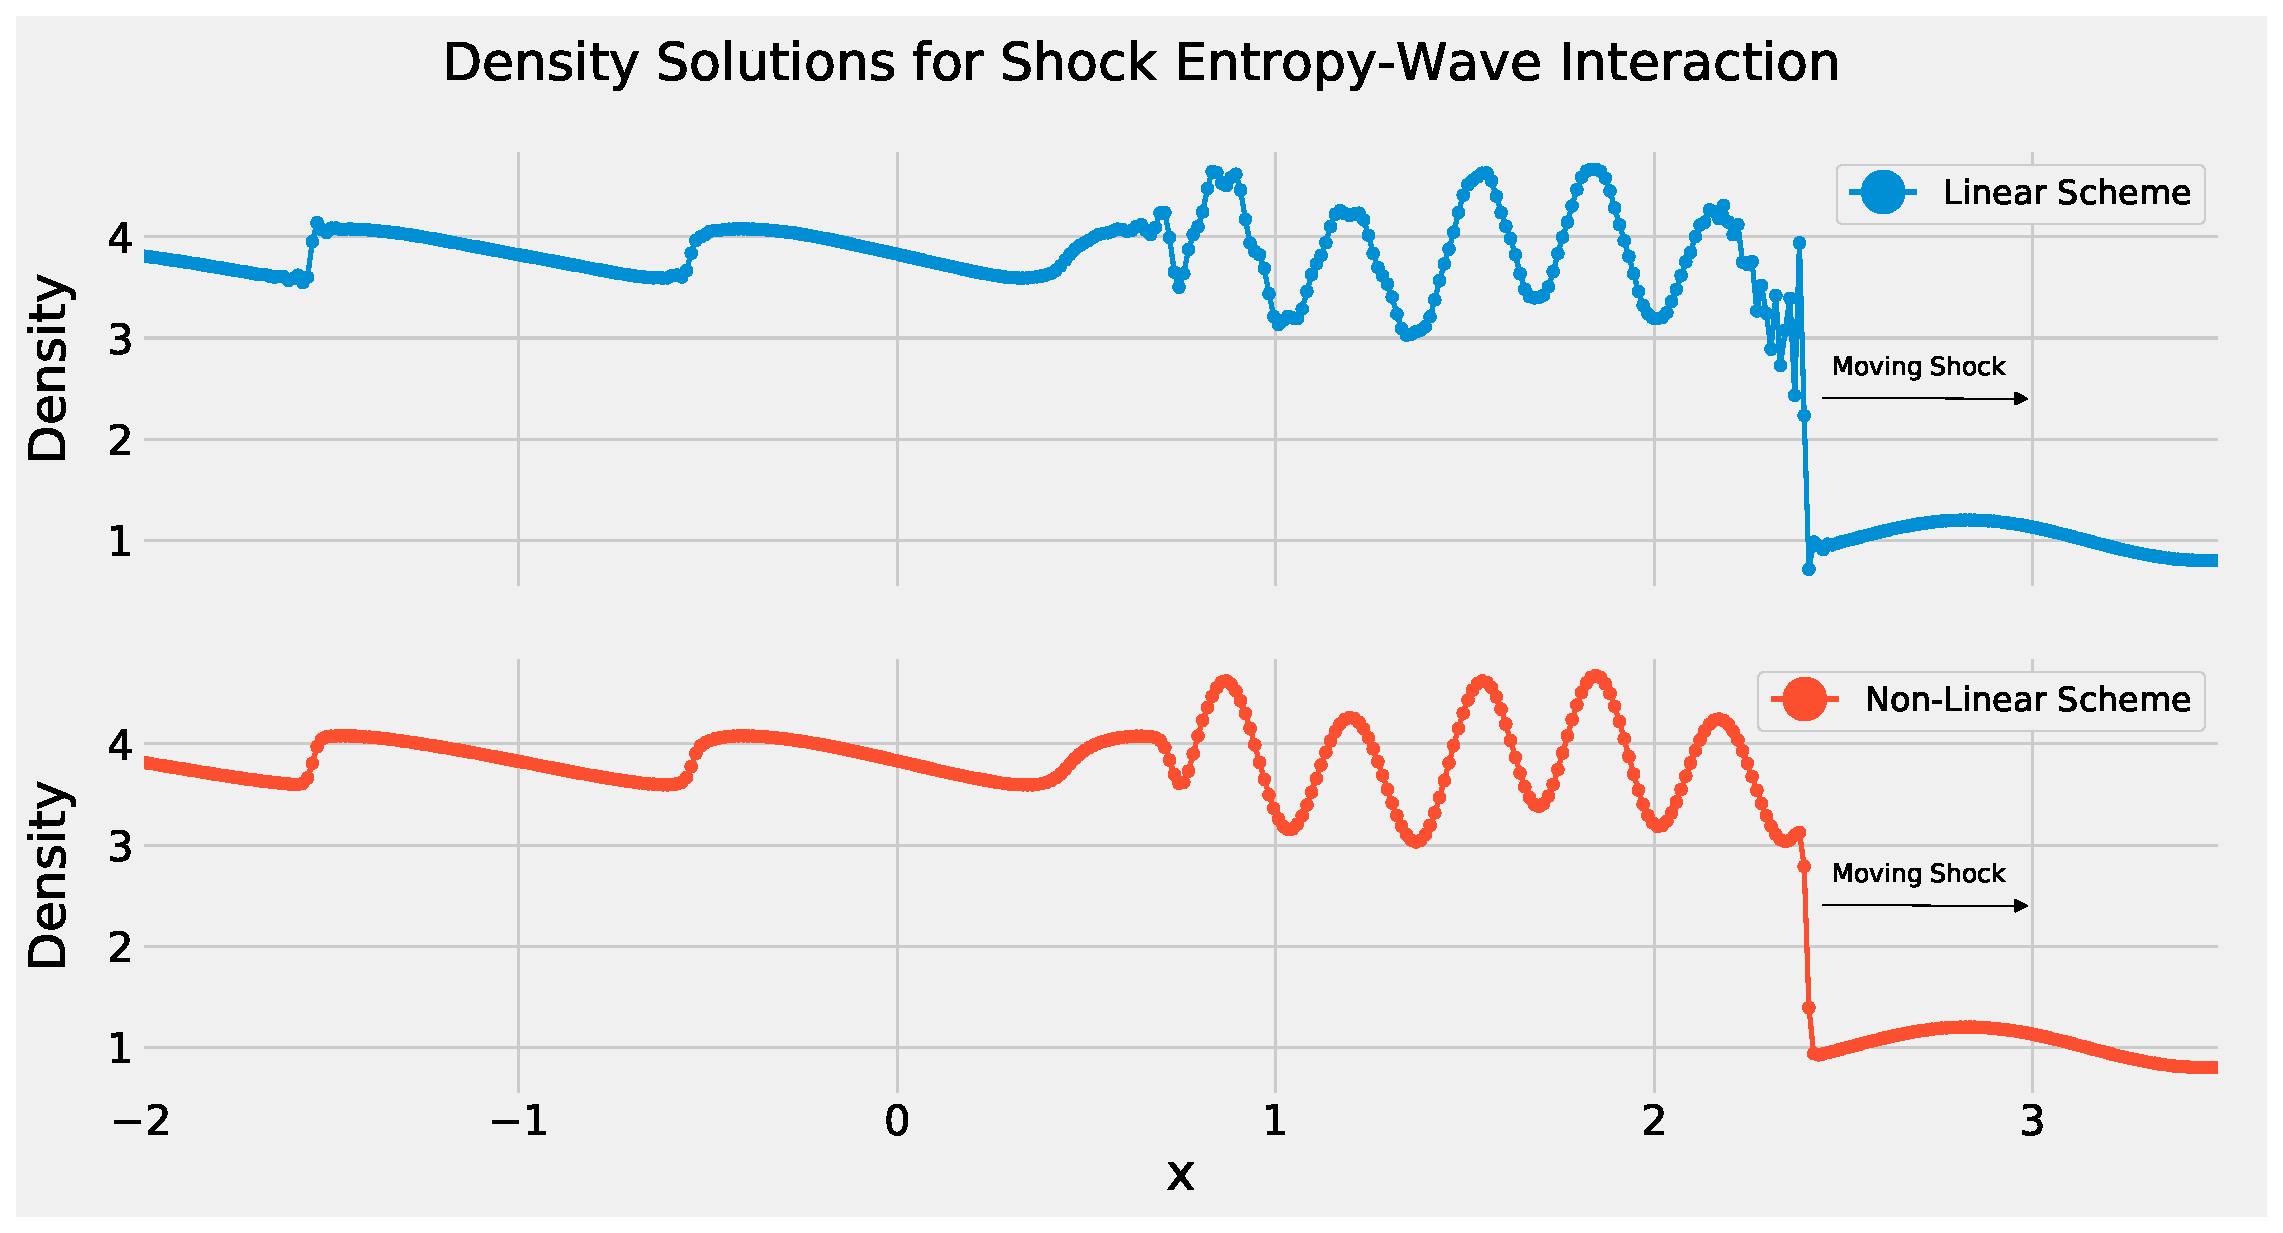
\includegraphics[scale=0.295]{DensitySolutions.eps}
  %   \end{figure}
  \begin{figure}[H]
    \centering
    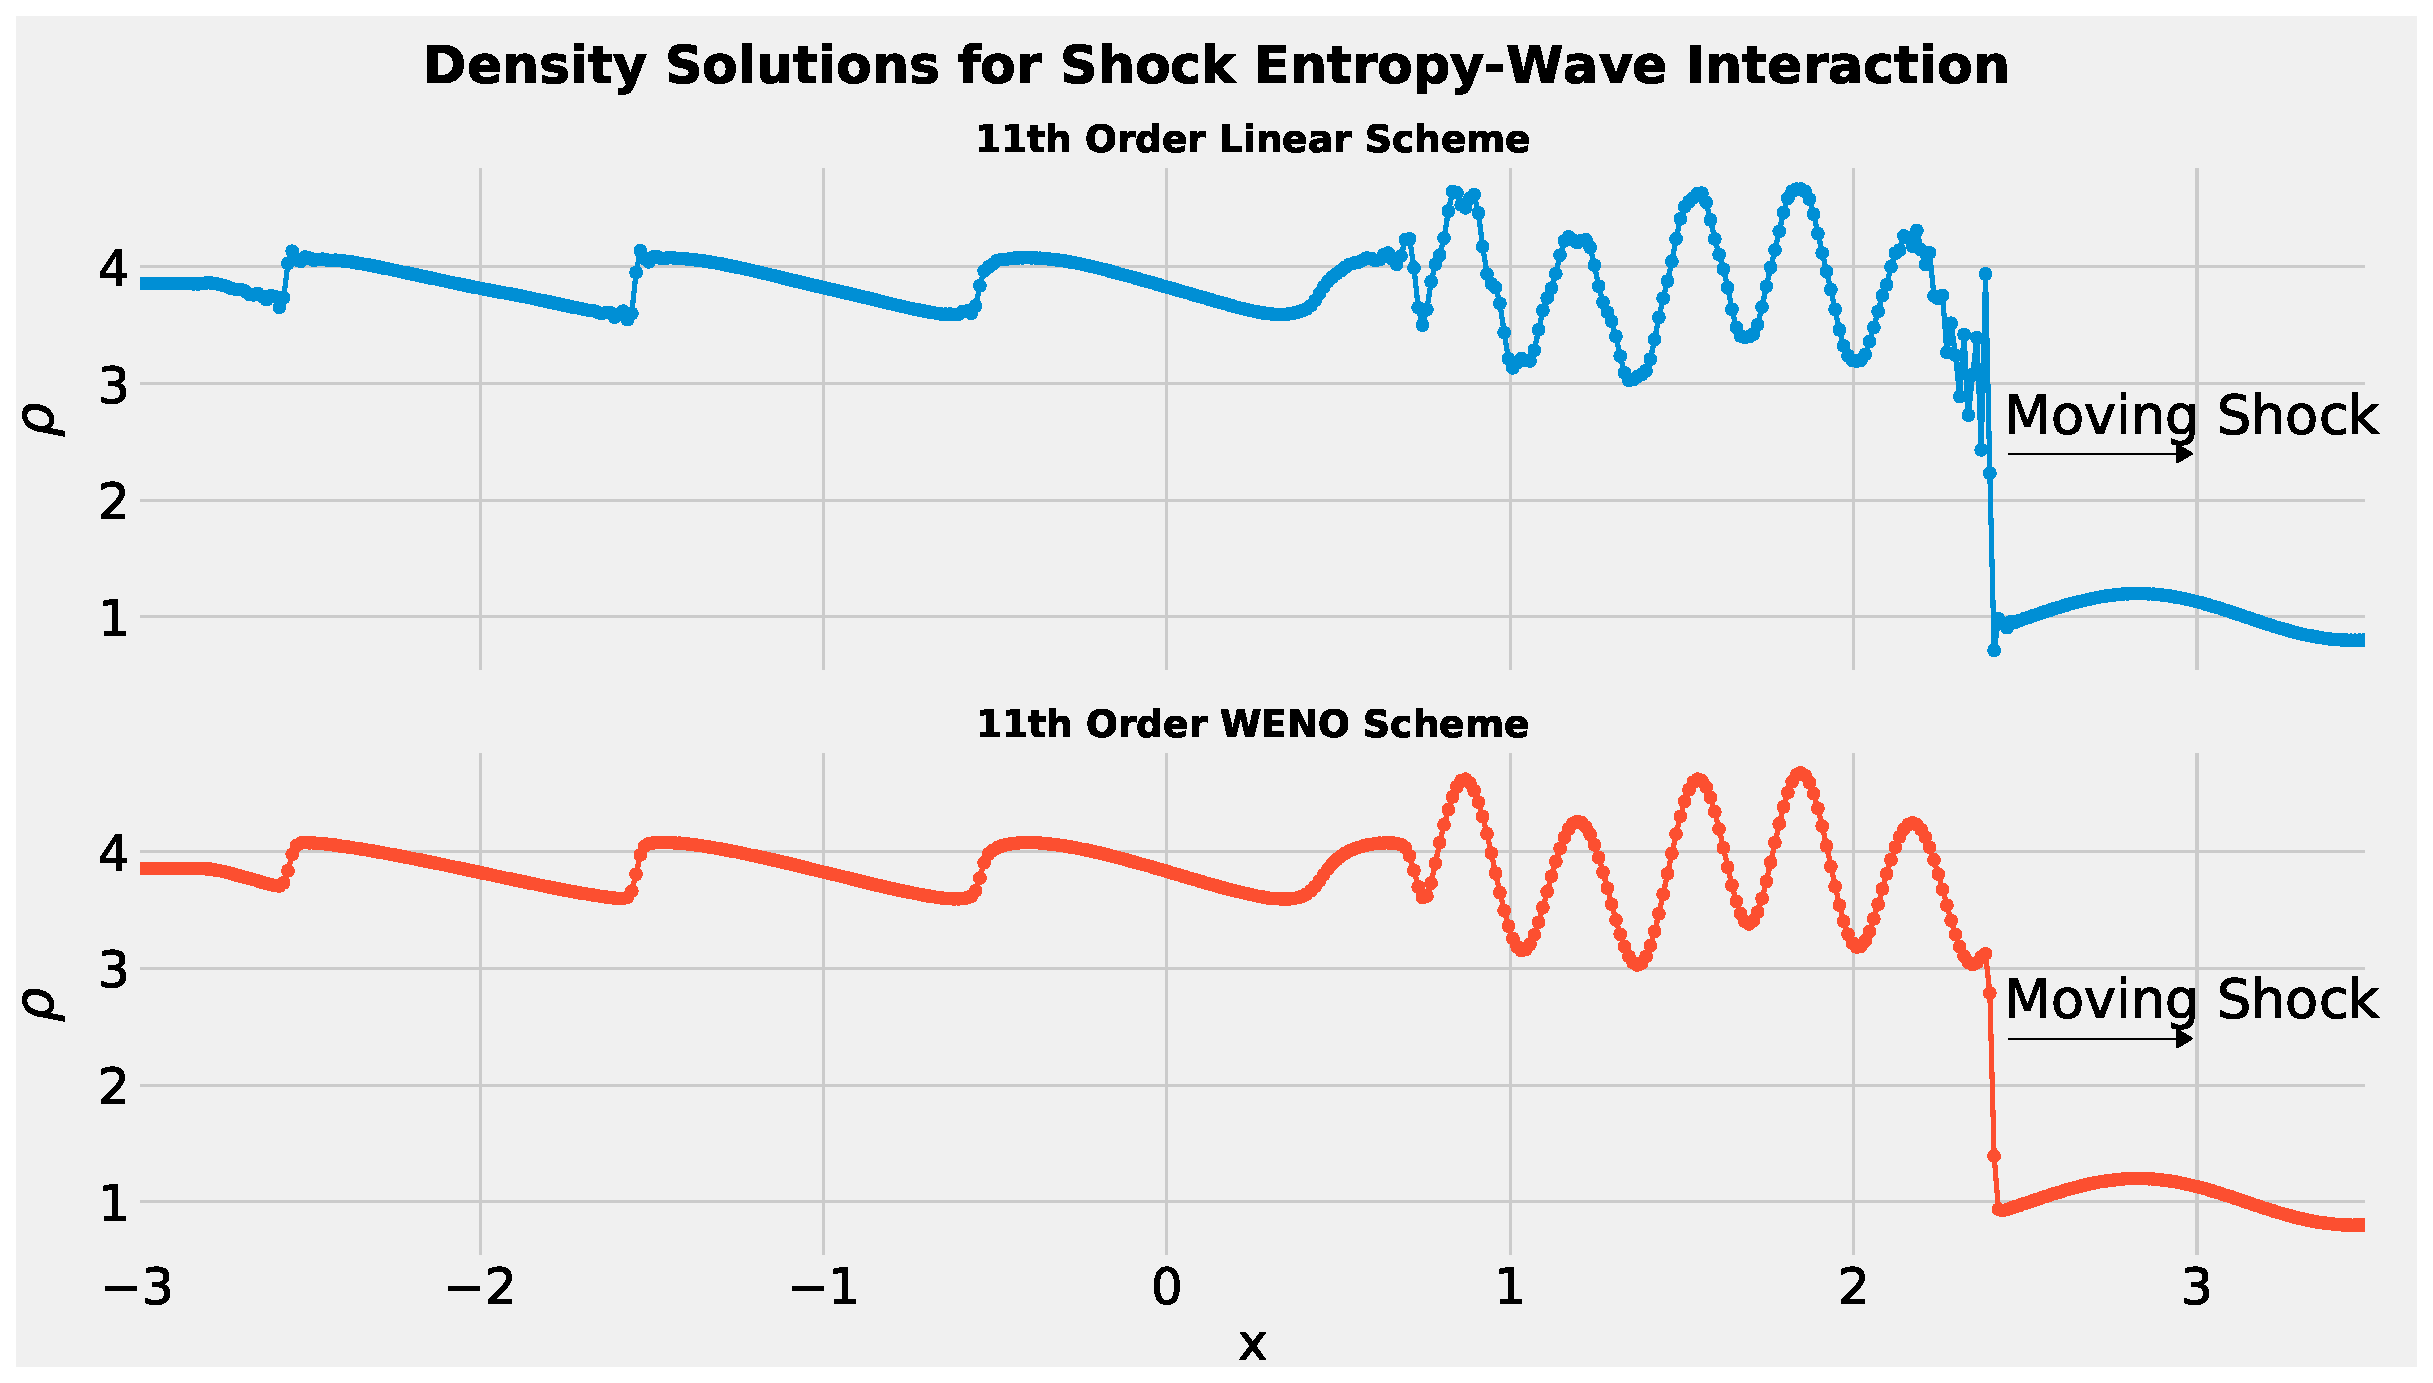
\includegraphics[scale=0.275]{ShockEntropyComparison.eps}
    \end{figure}
\end{frame}

\begin{frame}{Non-linear scheme for Euler Equations}
  \begin{itemize}
    \item The WENO scheme is designed to provide ``essentially" non-oscillatory behavior; small oscillations may be remain.
    \item For the Euler system, slight oscillations can result in negative density and/or pressure values which imply a non-real speed of sound
    \begin{itemize}
      \item[o] \textit{Complex sound speed results in simulation crashing.}
    \end{itemize}  
  \end{itemize}
  \textbf{To achieve a robust scheme, we need to enforce the positivity of density and pressure}
\end{frame}

\begin{frame}{Positivity Example}
  \begin{figure}[H]
    \centering
    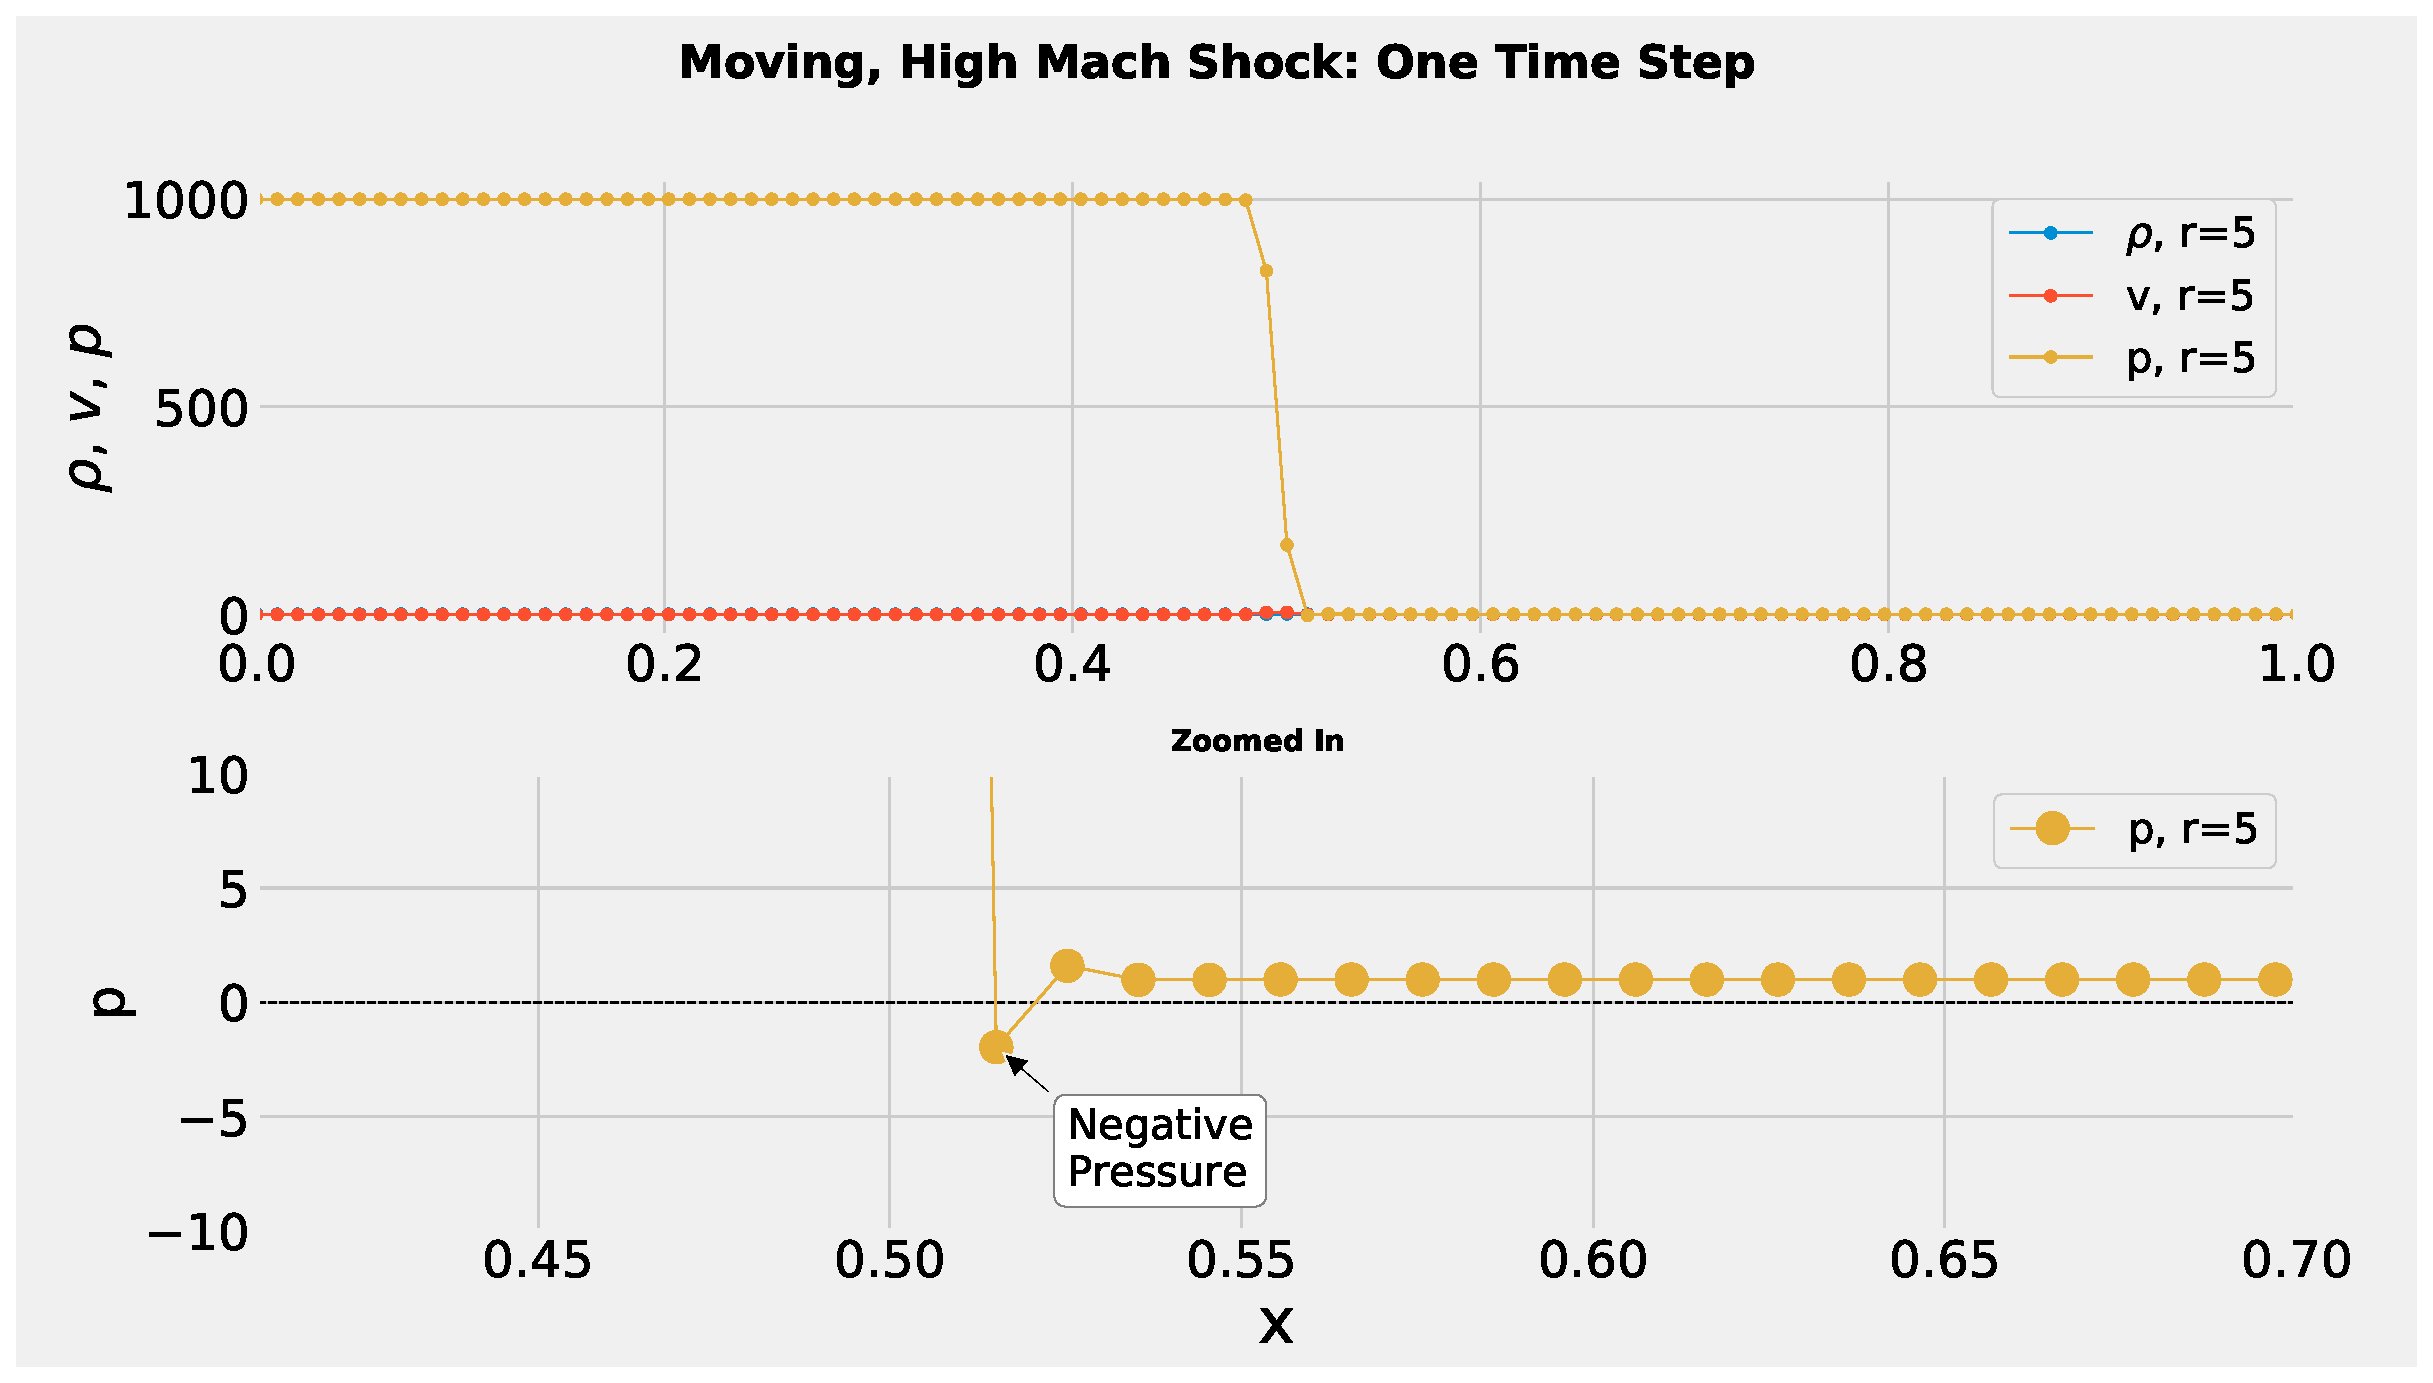
\includegraphics[scale=0.275]{PositivityZoom.eps}
    \end{figure}
  % $$u_i^{n+1}=u_i^n-\frac{\tau}{h}\{H^{RK}_{i,+} - H^{RK}_{i,-}\}$$
\end{frame}


\begin{frame}{Positivity Preserving Scheme}
  A positivity preserving scheme can be developed by combining the high order fluxes with the first order fluxes whenever necessary to prevent the solution from obtaining unphysical values.
  \begin{itemize}
    \item $h_{i+1/2}$: flux from first order method
    \item $H_{i+1/2}$: High order, WENO flux
  \end{itemize}
  
  The high order WENO approximation is of the form:
  $$
  \frac{\partial}{\partial x}[f(u_i)] = \frac{H_{i+1 /2} - H_{i-1/2}}{h}+\mathcal{O}(h^{2r-1})
  $$

  The first order approximation is:
  $$
  \frac{\partial}{\partial x}[f(u_i)] = \frac{h_{i+1 /2} - h_{i-1/2}}{h}+\mathcal{O}(h)
  $$
\end{frame}


\begin{frame}{Positivity Preserving Scheme}
  The positivity preserving scheme is realized by forming a modified flux (Xu, Mathematics of Computation, 2014): 
  $$\tilde{H}_{i+1/2}=h_{i+1/2} + \theta_{i+1/2}(H_{i+1/2} - h_{i+1/2})$$
  
  \begin{itemize}
    \item $\theta_{i+1/2} \in [0,1]$ are locally defined flux limiters.
    \item $\theta_{i+1/2} =1$ gives pure high order approximation
    \item $\theta_{i+1/2} =0$ gives first order
    \item For linear functions (e.g. density) $\theta_{i+1/2}$ are found by a sequence of 4 logical statements at each $i$. 
    \item Non-linear functions, e.g. pressure, require a root finding routine
  \end{itemize}

  The modified, high order, positivity preserving approximation is thus:
  $$
  \frac{\partial}{\partial x}[f(u_i)] \approx \frac{\tilde{H}_{i+1 /2} - \tilde{H}_{i-1/2}}{h}
  $$
\end{frame}

\begin{frame}{Positivity Example}
  Here we consider a problem consisting of a Mach 9.86 shock traveling through helium that interacts with a density interface:

  $$
  (\rho, v, p) = 
  \begin{cases} 
  (0.384,27.086,100.176)& \quad 0 \leq x < (0.5 - 2h) \\
  (0.1,0,1)& \quad (0.5 - 2h) \leq x \leq 0.5\\
  (100,0,1)& \quad  0.5 < x \leq 1
  \end{cases}
  $$
  \begin{figure}[H]
    \centering
    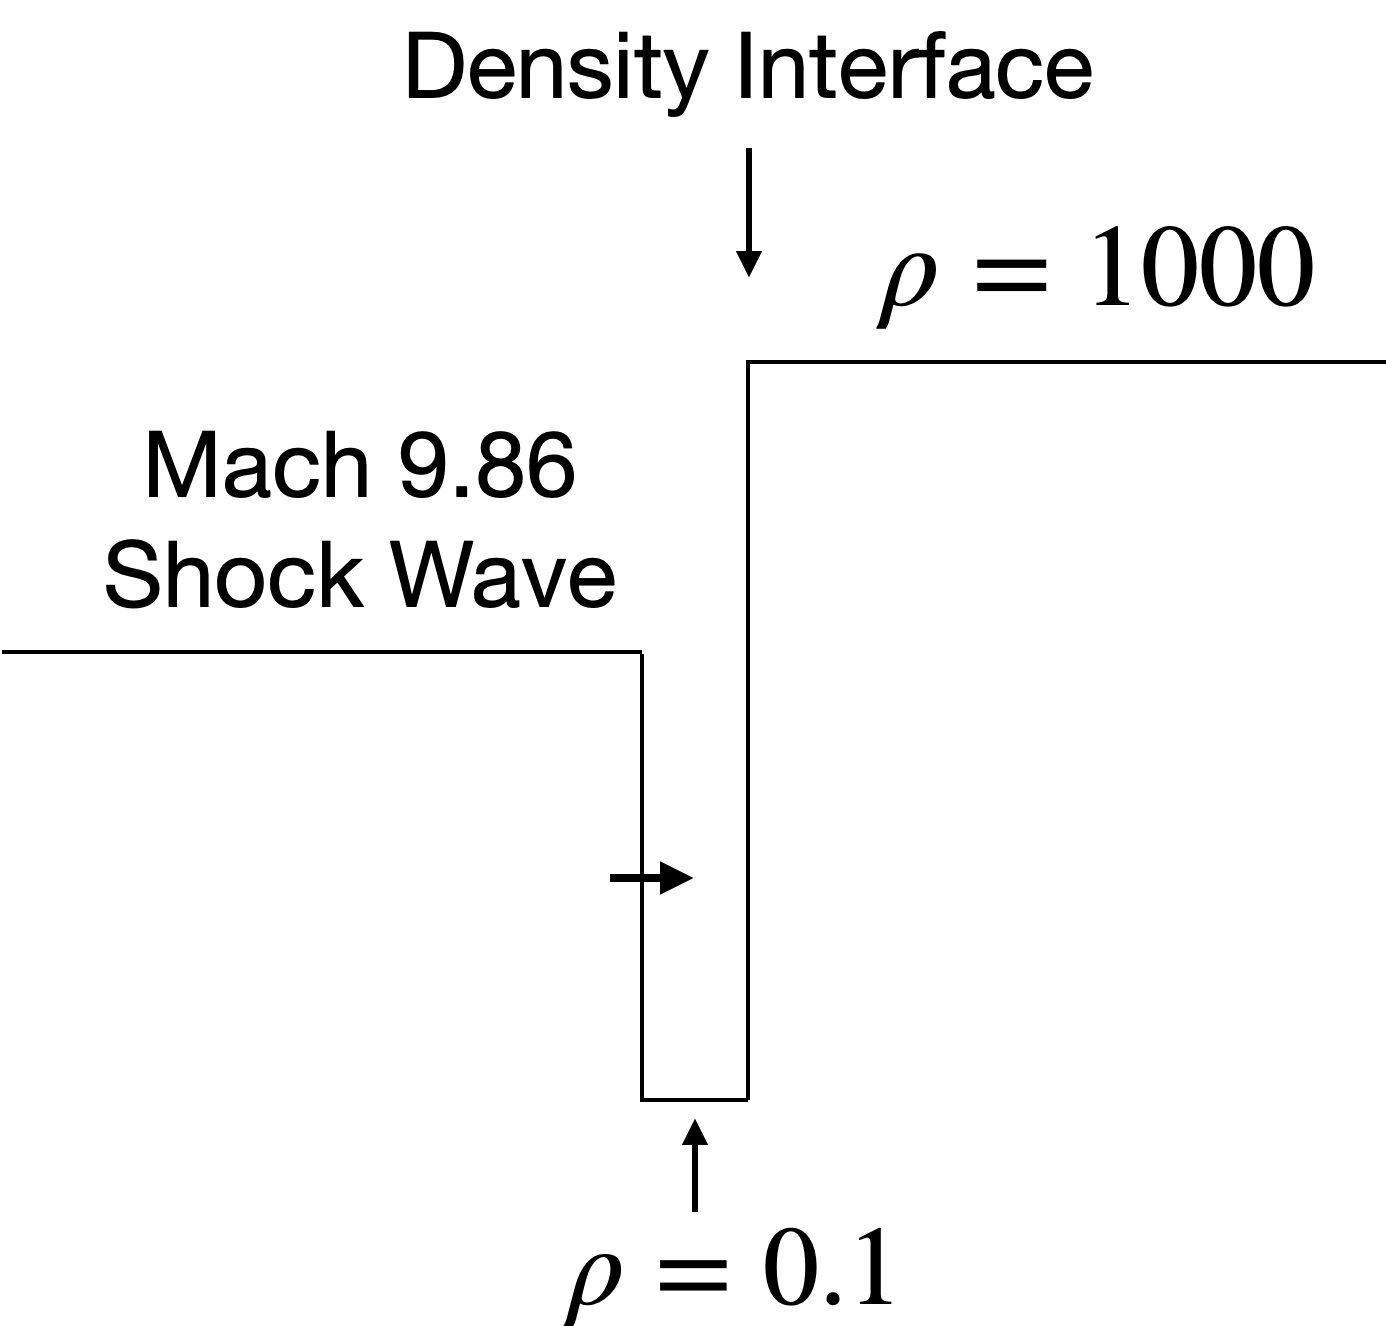
\includegraphics[scale=0.175]{ShockWave.png}
    \end{figure}
\end{frame}

\begin{frame}{Positivity Example}
  \begin{figure}[H]
    \centering
    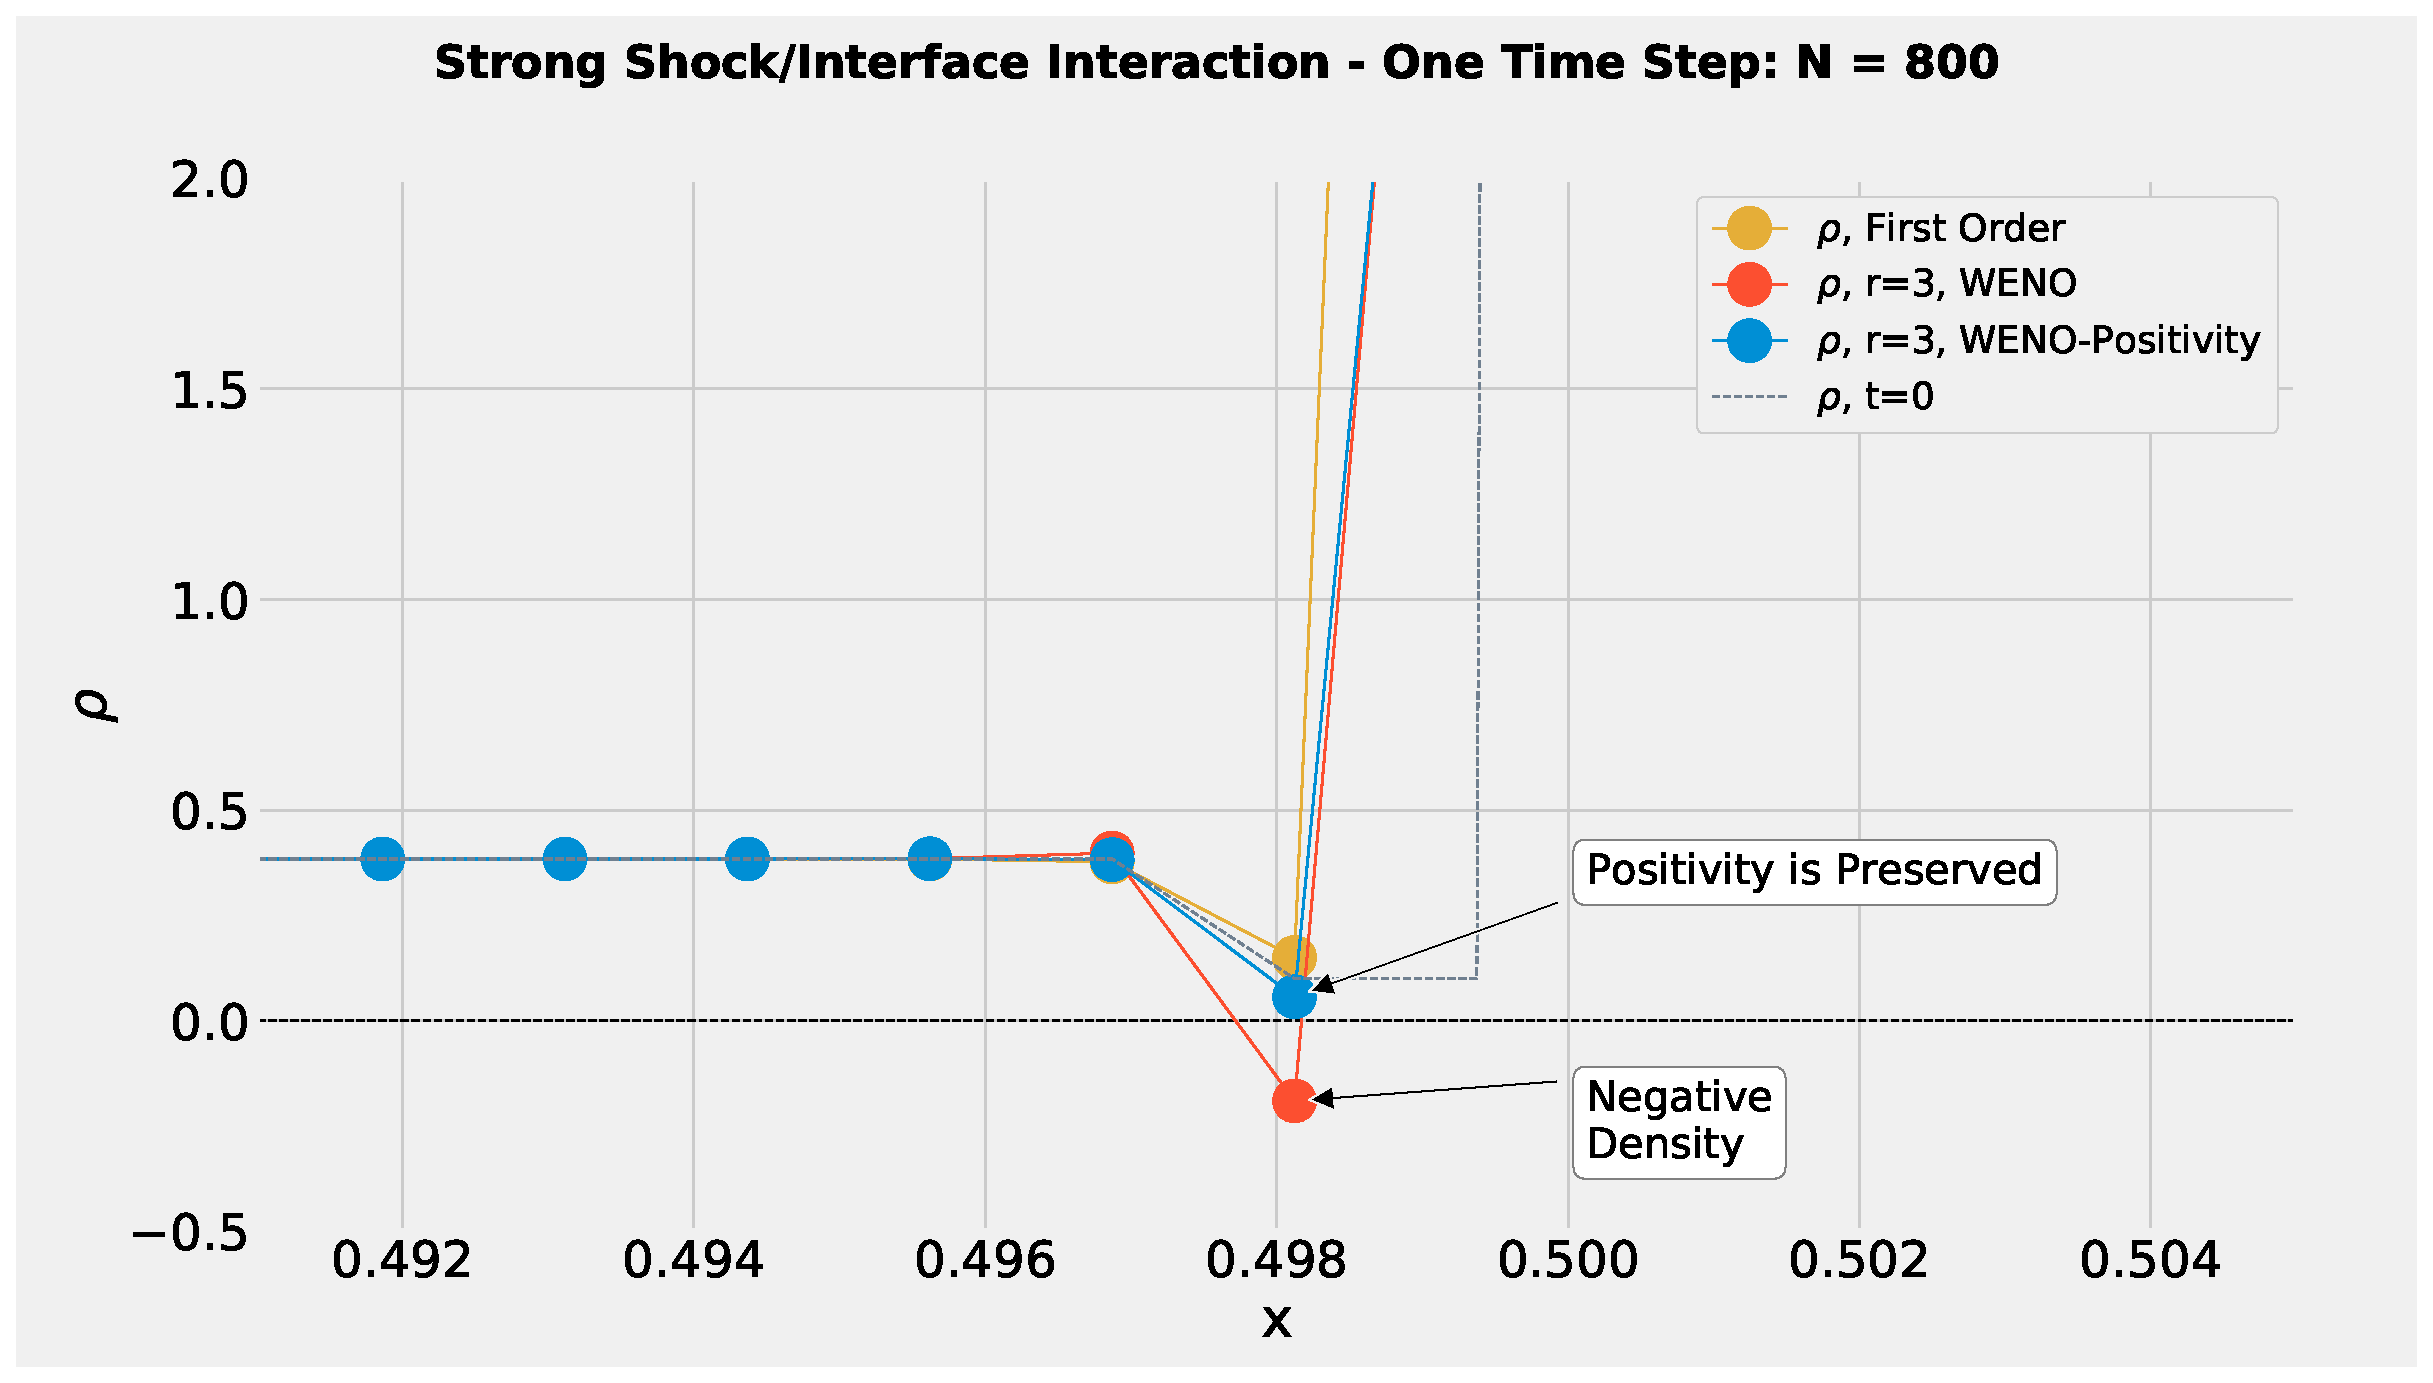
\includegraphics[scale=0.275]{PositivityZoomDenstiy.eps}
    \end{figure}
\end{frame}

\begin{frame}{Positivity Example}
  \begin{figure}[H]
    \centering
    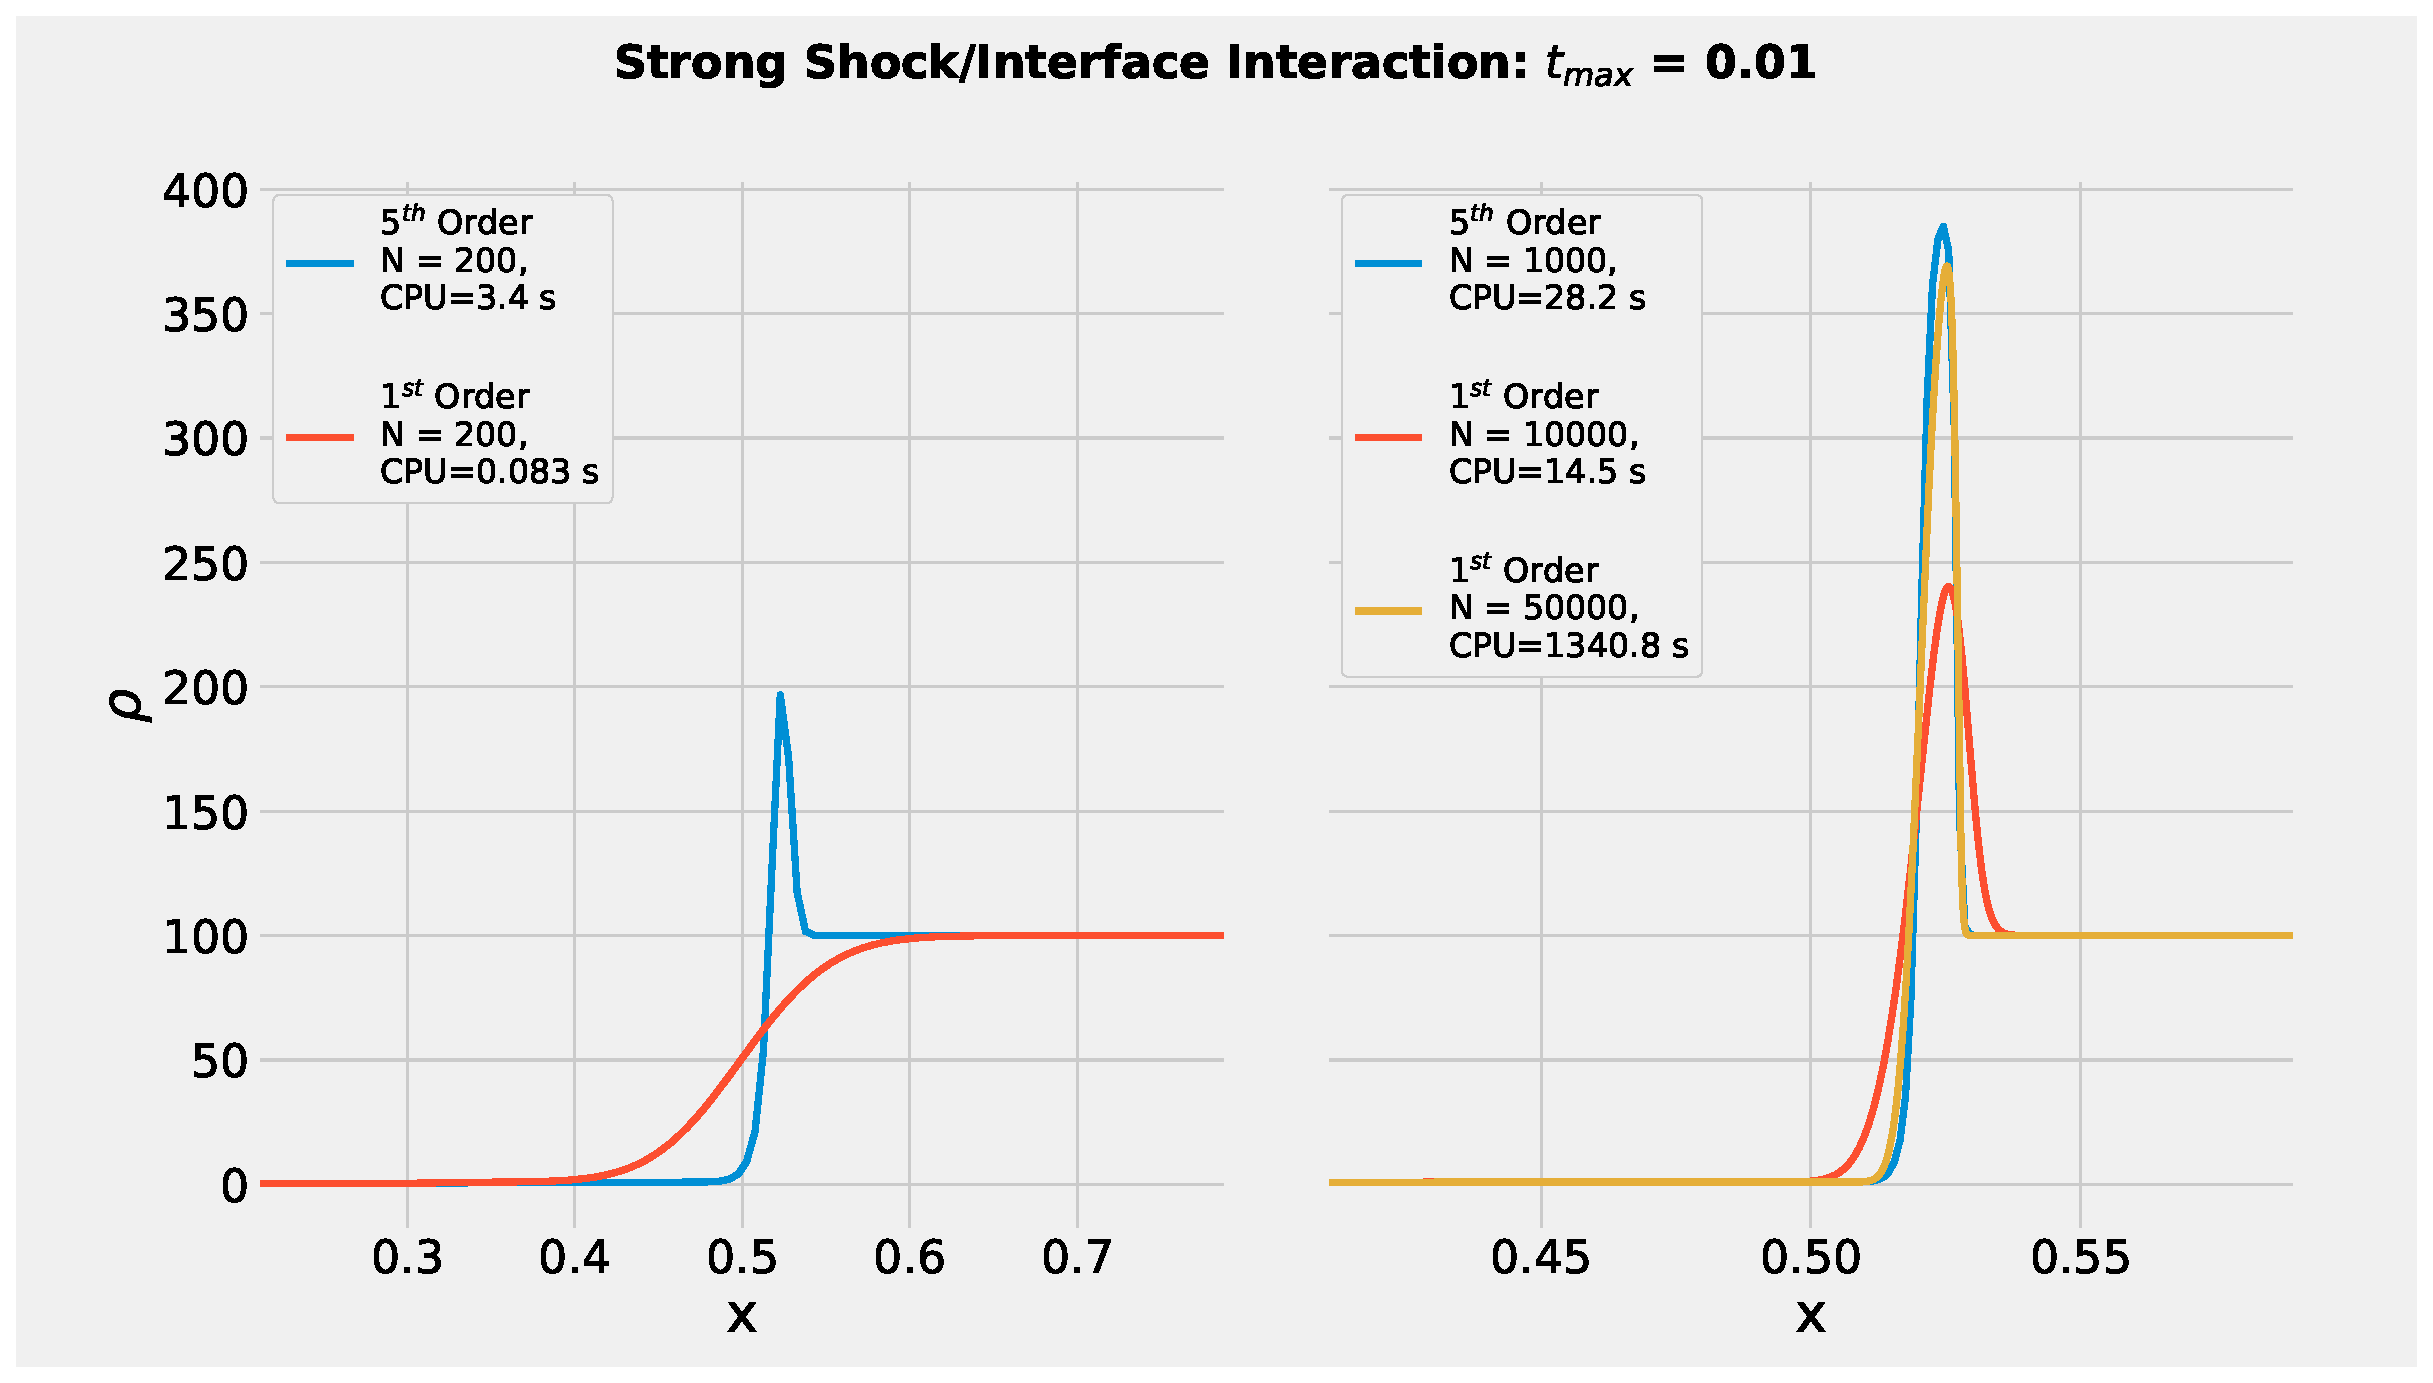
\includegraphics[scale=0.275]{ShockInterfaceComparison.eps}
    \end{figure}
\end{frame}

\begin{frame}{Two-fluid Positivity}
  To retain positivity within the two-fluid model we need to enforce the following (KS, unpublished):
  \begin{itemize}
    \item Upper and lower bounds of order parameters
    \item Positivity of density
    \item Positivity of a modified pressure $\frac{p+\Pi}{\gamma-1}$  
    \begin{itemize}
      \item[o] Ensures speed of sound is a real number
    \end{itemize}
  \end{itemize}
\end{frame}

\begin{frame}{Two-Fluid Positivity Implementation}
Two-fluid positivity is implemented using the flux limiting technique to form modified fluxes:
$$\tilde{H}_{i+1/2}=h_{i+1/2} + \theta_{i+1/2}(H_{i+1/2} - h_{i+1/2})$$
Because of the source terms in the order parameter equations, at each cell, we need to add the restriction of equal limiters (DB and KS, unpublished)
$$
\theta_{i+\frac{1}{2}} = \theta_{i-\frac{1}{2}} 
$$

\end{frame}

\begin{frame}{Two Fluid Positivity Example}
  \begin{figure}[H]
    \centering
    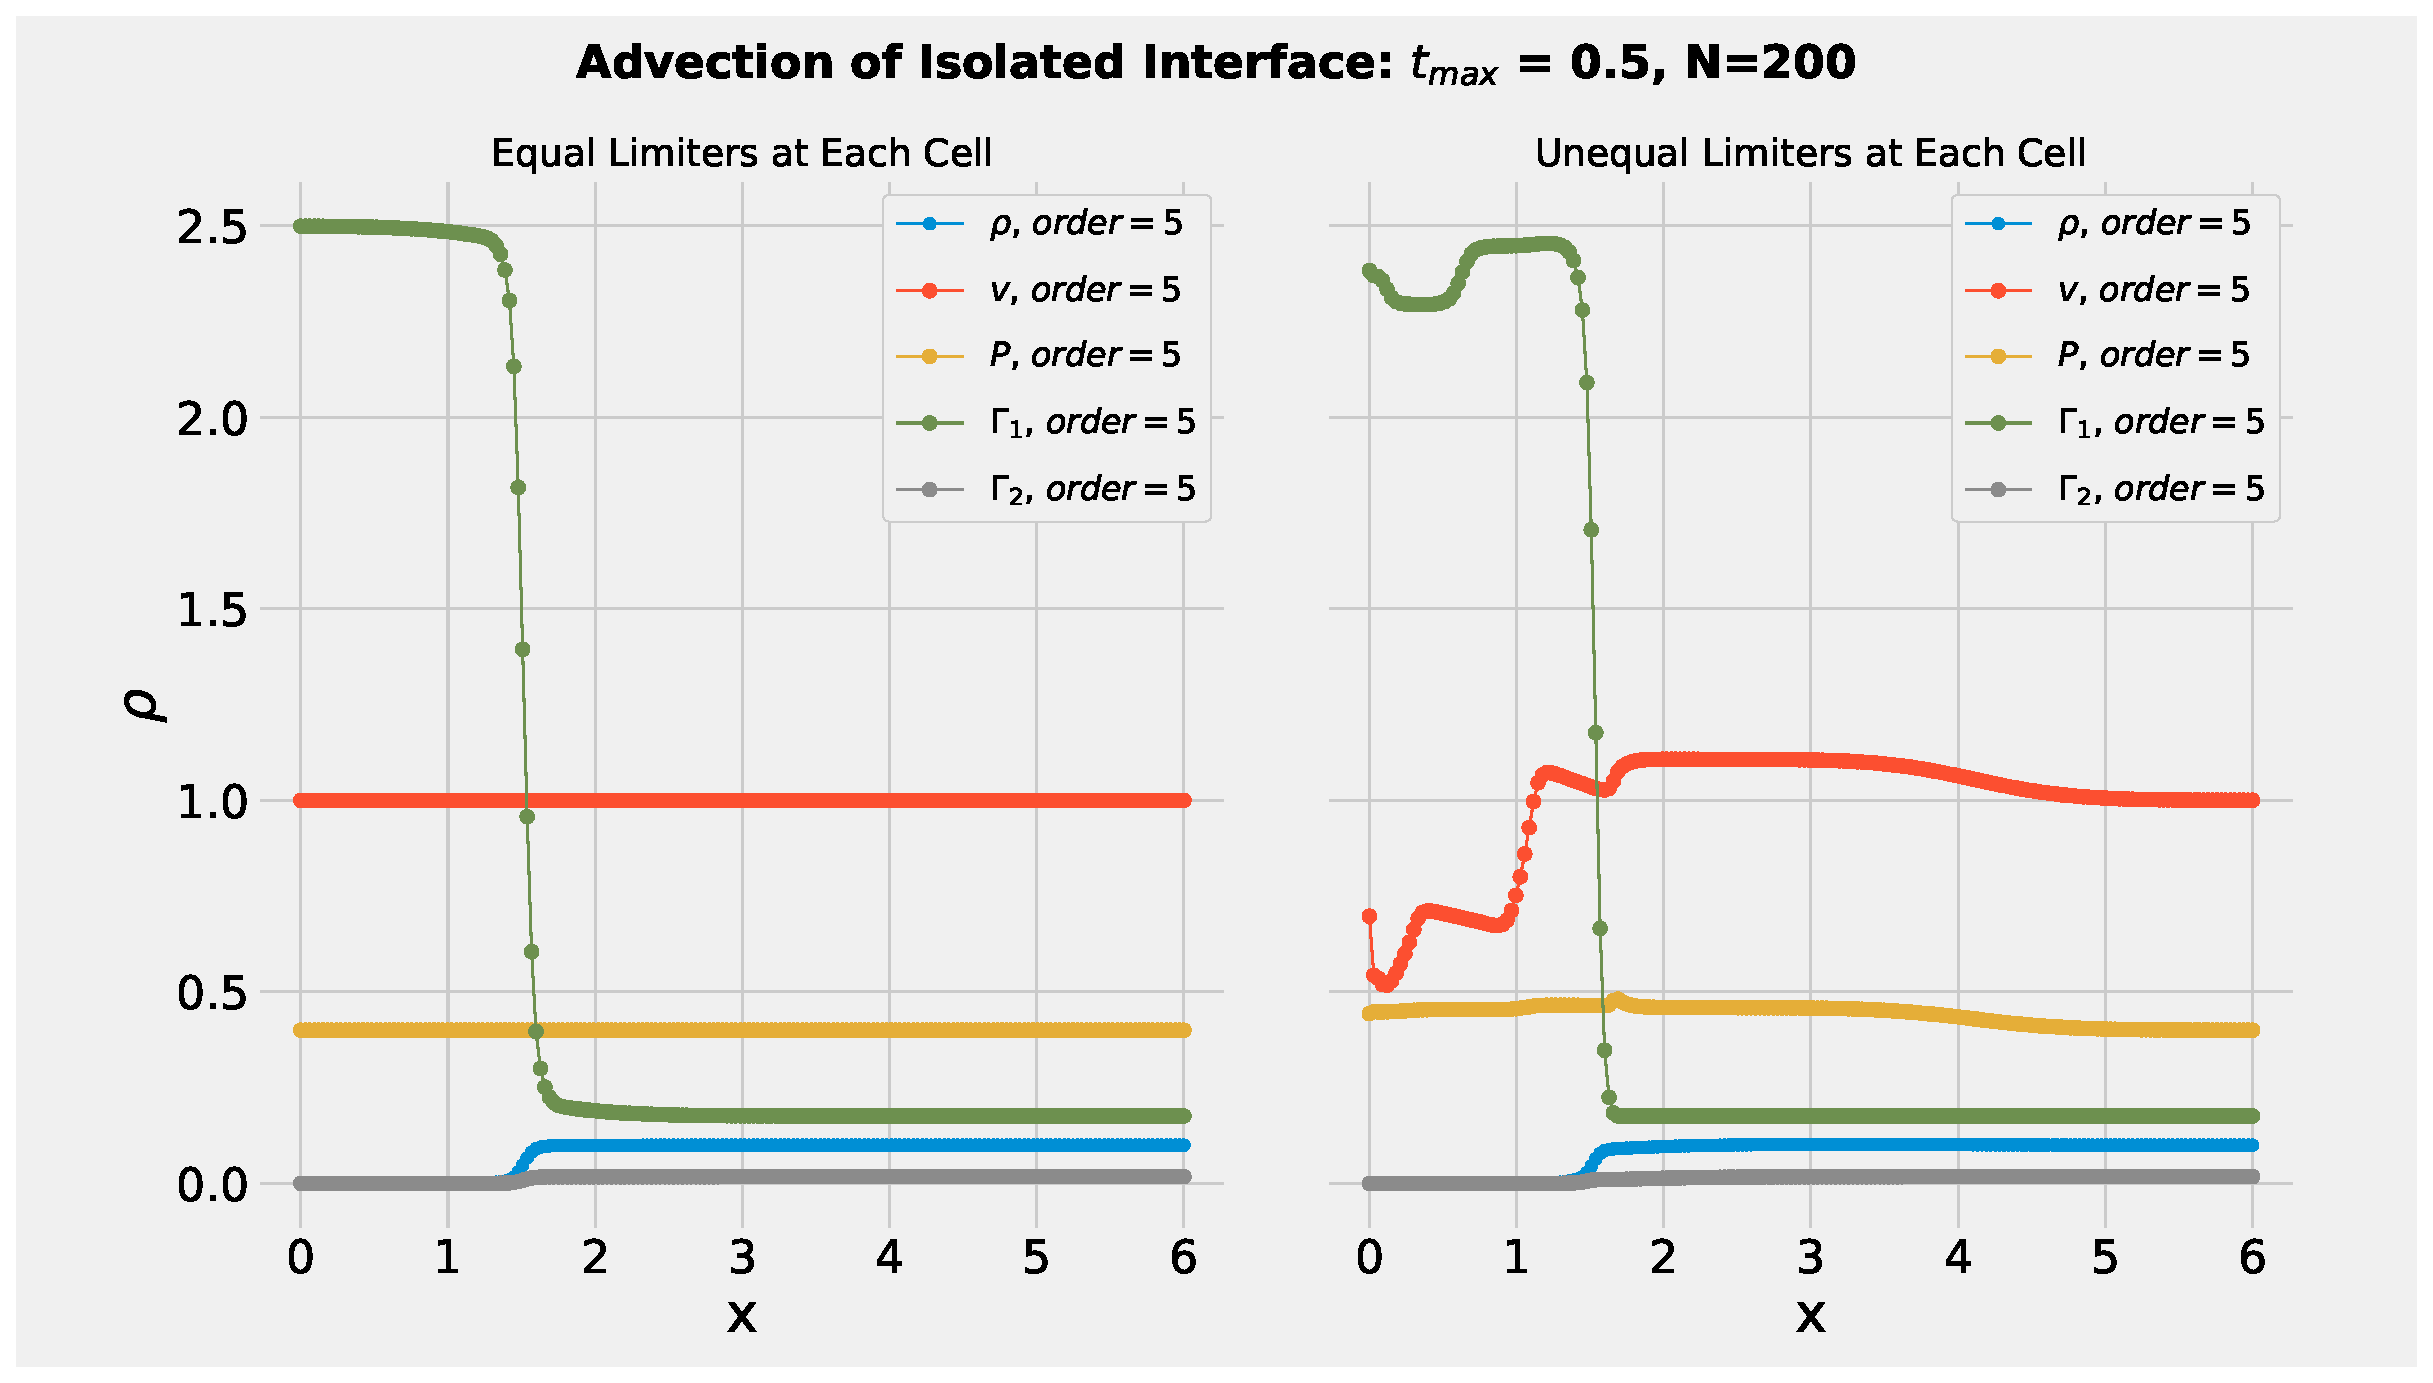
\includegraphics[scale=0.275]{TwoFluidComparison.eps}
    \end{figure}
\end{frame}


\begin{frame}{Conclusions and Ongoing Work}
  \textbf{Current Status}
\begin{itemize}
  \item A WENO finite difference scheme for two/phase fluid flow (KS, Computers and Fluids, 2019)
  \item Addition of positivity preservation for Euler System (DB and KS, unpublished)
\end{itemize}
\textbf{Ongoing Work}
\begin{itemize}
  \item Extend positivity preserving method to two-fluid problems 
\end{itemize}
\end{frame}

\begin{frame}{Acknowledgment}
  \begin{itemize}
  % \item
  %   Dr. Stanislav Emelianov, Georgia Tech.
  \item
    Office of Naval Research, contract $\#$ N000141712965
  \end{itemize}  
  
\end{frame}  

\appendix

\begin{frame}[allowframebreaks]{References}

  \bibliography{references.bib}
  \bibliographystyle{abbrv}

\end{frame}


\end{document}